\input ../talk-header.tex
\title{Machine Learning and AI}
\subtitle{Jour 1 : fondamentaux avancés}

\begin{document}

\begin{frame}
  \titlepage
\end{frame}

\talksection{Welcome}

\begin{frame}{Course structure}
  \only<1>{
    Two full days:
    \begin{itemize}
    \item  11, 12 July
    \end{itemize}
  }
  \only<2>{
    \begin{itemize}
    \item Email \url{jeff@p27.eu}
    \item Github: \url{https://github.com:JeffAbrahamson/ML-diva-beapp}
    \end{itemize}
  }
  \only<3>{
    \begin{itemize}
    \item Day 1 - ML theory
    \item Day 2 - ML Ops and Practices
    \end{itemize}
  }
\end{frame}

\begin{frame}
  \vphrase{Supervised}
\end{frame}

\begin{frame}
  \vphrase{Unsupervised}
\end{frame}

\begin{frame}
  \vphrase{Reinforcement}
\end{frame}

\begin{frame}
  \only<1>{
    \vphrase{Machine learning is not magic}
  }
  \only<2>{
    \vphrase{Machine learning is mathematics}
  }
  \only<3>{
    \vspace{1cm}
    \blue{\bf Mostly, it's these maths:}
    \begin{itemize}
    \item Probability
    \item Statistics
    \item Linear algebra
    \item Optimisation theory
    \item Differential calculus
    \end{itemize}
    \bigskip \purple{Unless you want to, we'll skip the maths.  For a
      certain definition of ``skip''.}  }
\end{frame}

\talksection{Probability}

\begin{frame}
  \frametitle{Probability}
  \phrase{events}
  \begin{itemize}
  \item Independence
  \item Dependence
  \item Bayes Theorem
  \end{itemize}
\end{frame}

\talksection{Statistics}

\begin{frame}[t]
  \frametitle{What is Statistics}

  \begin{enumerate}
  \item<1-3> Identify a question or problem.
  \item<1-3> Collect relevant data on the topic.
  \item<1-3> Analyze the data.
  \item<1-3> Form a conclusion.
  \end{enumerate}
  \only<2>{Sadly, sometimes people forget 1.}
  \only<3>{Statistics is about making 2--4 efficient, rigorous, and meaningful.}
  \only<3>{\vfill\prevwork{\textit{OpenIntro Statistics},
      2nd edition, D.~Diez, C.~Barr, M.~Çetinkaya-Rundel, 2013.}}
\end{frame}

\begin{frame}[t]
  \frametitle{What is data science?}

  \only<1-4>{(Exercise: Is this the same question as the last slide?)}

  \only<1>{
    \begin{enumerate}
    \item Define the question of interest
    \item Get the data
    \item Clean the data
    \item Explore the data
    \item Fit statistical models
    \item Communicate the results
    \item Make your analysis reproducible
    \end{enumerate}
  }
  \only<2>{
    \begin{enumerate}
    \item Define the question of interest
    \item Get the data
    \item Clean the data
    \item \purple{Explore the data}
    \item \purple{Fit statistical models}
    \item Communicate the results
    \item Make your analysis reproducible
    \end{enumerate}

    \blue{What the public thinks.}
  }
  \only<3>{
    \begin{enumerate}
    \item Define the question of interest
    \item \purple{Get the data}
    \item \purple{Clean the data}
    \item Explore the data
    \item Fit statistical models
    \item \purple{Communicate the results}
    \item \purple{Make your analysis reproducible}
    \end{enumerate}

    \blue{Where we spend most of our time.}
  }
  \only<4>{
    \begin{enumerate}
    \item \purple{Define the question of interest}
    \item Get the data
    \item Clean the data
    \item Explore the data
    \item Fit statistical models
    \item Communicate the results
    \item Make your analysis reproducible
    \end{enumerate}

    \blue{The easiest part to forget.}
  }
  \only<5>{\vfill\prevwork{\url{https://simplystats.github.io/2015/03/17/data-science-done-well-looks-easy}
      \url{-and-that-is-a-big-problem-for-data-scientists/}}}
\end{frame}

\begin{frame}
  \frametitle{Anecdote}

  Some properties of anecdote:

  \begin{itemize}
  \item is data
  \item haphazardly collected
  \item is generally not representative
  \item sometimes result of selective retention
  \item does not accumulate to be representative
  \item might be true (by chance)
  \item is ok to use as hypothesis, but be clear that hypothesis is anecdote
  \end{itemize}
\end{frame}

\begin{frame}
  \frametitle{Study Types}

  \begin{itemize}
  \item Observational
  \item Experimental
  \end{itemize}

  \only<2>{
    What can go wrong?
    \begin{itemize}
    \item Forgetting that association $\ne$ causation
    \item Not random
    \item Confounding variables
    \end{itemize}
  }
\end{frame}

\begin{frame}{Variables and statistics}
  \begin{itemize}
  \item Input: features (``explanatory variables'')
  \item Output: response variable
  \item Training set (learn parameters)
  \item Test Set (check learned parameters)
  \item Validation set (check learned hyperparameters)
  \item Cross validation (and jack knife and \dots)
  \item Bias and variance (picture coming up)
  \end{itemize}
\end{frame}

\begin{frame}
  \frametitle{Variable types}
  \cimg{images/variable-types.png}
\end{frame}

\begin{frame}
  \cimggg{images/bias-variance.png}
\end{frame}

\begin{frame}
  \frametitle{Mean}

  \begin{itemize}
  \item Weighted and unweighted
  \item Centroid to physicists
  \end{itemize}

  \only<2-4> {
    \cimgg{images/teeter-totter.png}
  }
  \only<3>{
    \begin{displaymath}
      \mu = E(X) = \sum w_i x_i = \mathbf{w\cdot x}
    \end{displaymath}

    \vfill
    \prevwork{\url{http://telescopes.stardate.org/images/research/teeter-totter/TT4.gif}}
  }
  \only<4>{
    \begin{displaymath}
      \mu = E(X) = \sum \Pr(X=x_i) x_i
    \end{displaymath}

    \vfill
    \prevwork{\url{http://telescopes.stardate.org/images/research/teeter-totter/TT4.gif}}
  }
  \only<5>{
    \begin{displaymath}
      \mu = E(X) = \int xf(x) \D{x}
    \end{displaymath}

    \vfill
    \prevwork{\url{http://telescopes.stardate.org/images/research/teeter-totter/TT4.gif}}
  }
  \only<6>{
    \cimgg{images/centroid-hanging-discrete.png}
  }
  \only<7>{
    \cimgg{images/centroid-balance-continuous.png}
  }
\end{frame}

\begin{frame}
  \frametitle{Population statistics}

  \only<1>{\vfill\centerline{\textbf{Mean} is just a sum.}
    \begin{displaymath}
      \mu = \frac{1}{N} \sum_{i=1}^N x_i
    \end{displaymath}

    \bigskip
    \centerline{This is a special case ($w_i=1$) of the weighted mean:}
    \begin{displaymath}
      \mu = \frac{1}{\sum w_i} \cdot \sum_{i=1}^N w_i x_i
    \end{displaymath}
  }
  \only<2>{\vfill\centerline{\textbf{Deviation} is distance from mean.}
    \begin{displaymath}
      \mu = \frac{1}{N} \sum_{i=1}^N x_i
    \end{displaymath}

    \begin{displaymath}
      \mbox{Deviation of } x_i = \mu - x_i
    \end{displaymath}
  }
  \only<3>{\vfill\centerline{\textbf{Variance} is the mean square of deviations}
    \begin{displaymath}
      \mu = \frac{1}{N} \sum_{i=1}^N x_i
    \end{displaymath}

    \begin{displaymath}
      \mbox{Var}(X) = \sigma^2 = \frac{1}{N} \sum_{i=1}^N (\mu - x_i)^2
    \end{displaymath}
  }
  \only<4>{\vfill\centerline{\textbf{Standard deviation} is square root of variance}
    \vfill
    \begin{displaymath}
      \mu = \frac{1}{N} \sum_{i=1}^N x_i
    \end{displaymath}

    \begin{displaymath}
      \sigma = \sqrt{\mbox{Var}(X)} = \sqrt{\sigma^2} = \sqrt{\frac{1}{N} \sum_{i=1}^N (\mu - x_i)^2}
    \end{displaymath}
  }
\end{frame}

\begin{frame}
  \cimghh{images/boxplot-vs-pdf.png}
\end{frame}

\begin{frame}
  \frametitle{Evaluating Normal Approximations}

  \only<1>{Easy technique 1: visually compare to normal plot.

    \cimghhh{images/normal-plot.png}
  }

  \only<2> {Easy technique 2: normal probability plot.

    \cimghhhh{images/normal-quantile.png}

    \vspace{-7mm}
    Also known as a quantile-quantile plot.
  }
\end{frame}

\begin{frame}
  \vfill
  \begin{displaymath}
    \overline{x}\ne\mu
  \end{displaymath}
  \vfill
\end{frame}

\begin{frame}
  \frametitle{Inference Concepts}

  \only<1->{\textbf{Running mean.}  Sequence of partial sums (divided
    by number in sum).
  }

  \only<2>{
    \bigskip
    \cimgg{images/running-mean.png}
  }

  \only<3->{\textbf{Sampling variation.}  Change of $\overline x$ from
    one sample to the next.
  }

  \only<4->{\textbf{Sampling distribution.}  The distribution of
    possible point samples of a fixed size from a given population.
  }
\end{frame}

\begin{frame}{Inference Concepts}
    \begin{itemize}
    \item Law of large numbers
    \item Central limit theorem
    \end{itemize}
\end{frame}

\begin{frame}
  \frametitle{Sampling distribution}

  \cimg{images/sampling-distribution.png}
\end{frame}

\begin{frame}
  \frametitle{Confidence intervals}

  Sample $n$ points, choose an interval around the sample mean.

  A 95\% confidence interval means if we sample repeatedly, about 95\%
  of the samples will contain the population mean.

  \only<2>{
    \cimghhhh{images/confidence-intervals.png}
  }

  \only<3>{
    \cimghhhh{images/confidence-intervals-2.png}
  }
\end{frame}


\talksection{Linear Algebra}

\begin{frame}
  \vphrase{Vector Space}
\end{frame}

\begin{frame}
  \vphrase{Curse of Dimensionality}
\end{frame}

\begin{frame}
  \frametitle{Linear algebra: basics}
  \only<1>{
    \begin{displaymath}
      v =
      \begin{pmatrix}
        v_1\\
        v_2\\
        \vdots\\
        v_n
      \end{pmatrix}
      \in \mathbb{R}^n
    \end{displaymath}

    \bigskip
    This is all mostly for convenience (not getting lost).  Remember weighted averages?
    \begin{displaymath}
      \mu = w^T\cdot x
    \end{displaymath}
  }
  \only<2>{
    \begin{align*}
      A & =
      \begin{bmatrix}
        a_{1,1} & a_{1,2} & a_{1,3} \\
        a_{2,1} & a_{2,2} & a_{2,3} \\
        a_{3,1} & a_{3,2} & a_{3,3}
      \end{bmatrix}
      =
      \begin{pmatrix}
        a_{1,1} & a_{1,2} & a_{1,3} \\
        a_{2,1} & a_{2,2} & a_{2,3} \\
        a_{3,1} & a_{3,2} & a_{3,3}
      \end{pmatrix} \\[4mm]
      & =
      \begin{Bmatrix}
        a_{1,1} & a_{1,2} & a_{1,3} \\
        a_{2,1} & a_{2,2} & a_{2,3} \\
        a_{3,1} & a_{3,2} & a_{3,3}
      \end{Bmatrix}
      \in \mathbb{R}^{n\times n}
    \end{align*}
  }
  \only<3>{
    \begin{displaymath}
        u + v =
      \begin{pmatrix}
        u_1 + v_1\\
        u_2 + v_2\\
        \vdots\\
        u_n + v_n
      \end{pmatrix}
    \end{displaymath}
  }
  \only<4>{
    \begin{displaymath}
      \alpha v =
      \begin{pmatrix}
        \alpha v_1\\
        \alpha  v_2\\
        \vdots\\
        \alpha v_n
      \end{pmatrix}
       \qquad (\alpha\in\mathbb{R})
    \end{displaymath}
  }
  \only<5>{
    \begin{displaymath}
      \parallel v\parallel = \sqrt{v_1^2 + \cdots + v_n^2}
    \end{displaymath}
  }
  \only<6>{
    \begin{align*}
      u\cdot v & = u_1\cdot v_1 + \dotsb + u_n \cdot v_n \\[4mm]
      & = \parallel u\parallel \parallel v\parallel \cos\theta
    \end{align*}
  }
  \only<7>{
    \begin{align*}
      C = A + B & \iff c_{ij} = a_{ij} + b_{ij} \\[5mm]
      %
      C = AB & \iff c_{ij} = \sum_k a_{ik}b_{kj} \\[5mm]
      %
      A = B^T & \iff a_{ij} = b_{ji}
    \end{align*}

    \begin{displaymath}
      AA^{-1} = A^{-1}A = \mathrm{diag}(1)
    \end{displaymath}
  }
\end{frame}

\begin{frame}
  \frametitle{Linear algebra: transformations}
  \only<1>{
    \begin{align*}
      Ax = y & \hspace{1cm} f = T_A \,:\, \mathbb{R}^n\rightarrow \mathbb{R}^n \\[5mm]
      %
      x = A^{-1}Ax = A^{-1}y & \hspace{1cm} f^{-1} = T_{A^{-1}}
      \,:\, \mathbb{R}^n\rightarrow \mathbb{R}^n \\[5mm]
    \end{align*}
  }
  \only<2-3>{
    $B$ is a basis for $V$ iff any of these conditions are met:
    \begin{itemize}
    \item $B$ is a minimal generating set of $V$
    \item $B$ is a maximal set of linearly independent vectors
    \item Every vector $v\in V$ can be expressed in a unique way as a sum of $b_i\in B$
    \end{itemize}

    \purple{(The conditions are equivalent.)}

    \only<3>{\red{Bases are not unique.}}
  }
  \only<4-6>{Eigenvectors, eigenvalues:
    \begin{displaymath}
      Av = \lambda v
    \end{displaymath}

    \only<5>{
      \begin{displaymath}
        Av = \lambda 1 v \;\iff\; (A-\lambda 1)v = 0
      \end{displaymath}
    }
    \only<6>{
      Some matrices are diagonalisable.  Then
      \begin{align*}
        A = Q\Lambda Q^{-1} \hspace{1cm} \mbox{ with } \Lambda & =
        \begin{bmatrix}
          \lambda_1 & \cdots & 0 \\
          \vdots & \ddots & 0 \\
          0 & 0 & \lambda_n
        \end{bmatrix} \\[5mm]
        %
        \mbox{and } Q & =
        \begin{bmatrix}
          \mid && \mid \\
          v_1 & \cdots & v_n \\
          \mid && \mid
        \end{bmatrix}
      \end{align*}
    }
  }
  \only<7>{\vphrase{video time}}
\end{frame}

%%%%%%%%%%%%%%%%%%%%%%%%%%%%%%%%%%%%%%%%%%%%%%%%%%%%%%%%%%%%%%%%%%%%%%
%\talksection{Break}

\talksection{Features}

\begin{frame}
  \vphrase{Features and Modeling}
\end{frame}

\begin{frame}
  \phrase{Vector spaces}

  \vspace{1cm}
  \only<2>{\centerline{Features are dimensions}}
\end{frame}

\begin{frame}
  \phrase{Feature extraction}

  \vspace{1cm}
  \phrase{Feature engineering}

  \only<2>{\vspace{3mm}\centerline{Synthetic features}}
\end{frame}

\begin{frame}
  \frametitle{Feature Engineering}
  \only<1>{
    \begin{enumerate}
    \item Brainstorm
    \item Pick some
    \item Make them
    \item Evaluate
    \item Repeat
    \end{enumerate}
  } \purple{This is most often done with neural nets these days, but
    the technique is still useful.}
\end{frame}

\begin{frame}
  \vphrase{One of $K$ = one-hot encoding}
\end{frame}

\begin{frame}
  \frametitle{Text features}
  \blue{Bag of words}
  \only<1>{
    \begin{itemize}
    \item Corpus (documents)
    \item Vocabulary (set of unique words)
    \item Words
    \end{itemize}
  }
  \only<2>{
    \begin{itemize}
    \item Order doesn't matter
    \item Stop words
    \item Stemming {\it(racinisation, désuffixation)}
    \item Lemmatisation {\it(transformer en lemme)}
    \end{itemize}
  }
\end{frame}

\begin{frame}
  \frametitle{Image features}
  \only<1>{
    \begin{itemize}
    \item Corners, edges (rotation invariant, but scaling can hide)
    \item More complex: scale space or RNN
    \item Point matching is easy
    \end{itemize}
    \purple{Since 2012 or so, this is mostly done by neural networks.}
  }
  \only<2>{
    Problems
    \begin{itemize}
    \item Illumination
    \item Scale
    \item Rotation
    \item Skew (perspective)
    \item Data size (matrices not sparse)
    \end{itemize}
  }
\end{frame}

\begin{frame}
  \frametitle{python}
  \only<1>{Useful tools
    \begin{itemize}
    \item virtualenv
    \item pip
    \item ipython
    \item jupyter notebook
    \item \url{conda.pydata.org}
    \end{itemize}
  }
  \only<2>{Notes
    \begin{itemize}
    \item \texttt{pip install -r requirements.txt}
    \item ipython offers tab completion (vs python)
    \item jupyter notebook opens in a browser, caches cell output but not cell state
    \end{itemize}
  }
\end{frame}

\begin{frame}
  \frametitle{pandas}
  \only<1>{\lstinputlisting{code/pandas_1.py}}
  \only<2>{\purple{\texttt{Dataframe} has many constructors.  For example,}
    \lstinputlisting{code/pandas_2.py}
  }
  \only<3>{\purple{Viewing data}
    \lstinputlisting{code/pandas_3.py}
  }
  \only<4>{\purple{Basic data exploration}
    \lstinputlisting{code/pandas_4.py}
  }
  \only<5>{\purple{Select a column (series)}
    \lstinputlisting{code/pandas_5.py}
  }
  \only<6>{\purple{Select a range}
    \lstinputlisting{code/pandas_6.py}
  }
  \only<7>{\purple{Boolean selection criteria}
    \lstinputlisting{code/pandas_7.py}
  }
  \only<8>{\purple{Recommended}

    \vspace{5mm}
    \url{http://www.gregreda.com/2013/10/26/intro-to-pandas-data-structures/}
  }
\end{frame}

\begin{frame}
  \frametitle{Plotting}
  \only<1>{\purple{Draw a line}
    \lstinputlisting{code/pyplot_1.py}
    \vspace{-19mm}
    \flushright{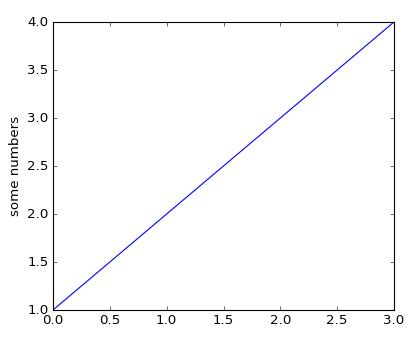
\includegraphics[width=.5\textwidth]{images/pyplot_1.png}}
  }
  \only<2>{\purple{Draw a line}
    \lstinputlisting{code/pyplot_2.py}
    \vspace{-19mm}
    \flushright{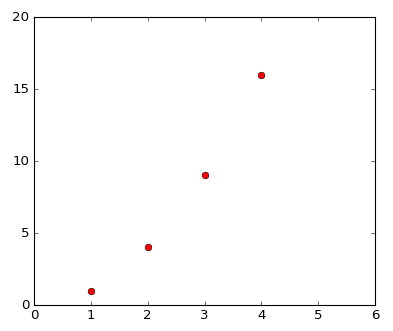
\includegraphics[width=.5\textwidth]{images/pyplot_2.png}}
  }
  \only<3>{\purple{Draw a line}
    \lstinputlisting{code/pyplot_3.py}
    \vspace{-55mm}
    \flushright{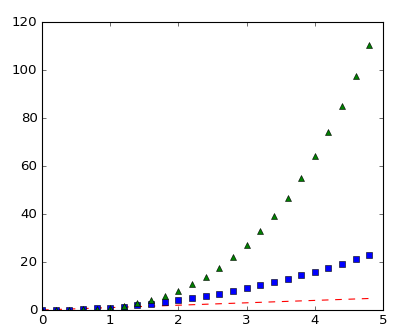
\includegraphics[width=.5\textwidth]{images/pyplot_3.png}}
  }
  \only<4>{\purple{Draw two curves}
    \lstinputlisting{code/pyplot_4.py}
  }
  \only<5>{
    \flushright{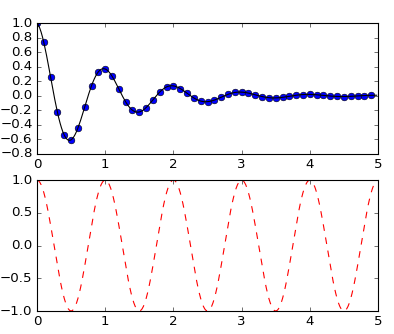
\includegraphics[width=.5\textwidth]{images/pyplot_4.png}}
  }
  \only<6>{\purple{Draw two curves}
    \lstinputlisting{code/pyplot_5.py}
  }
  \only<7>{
    \flushright{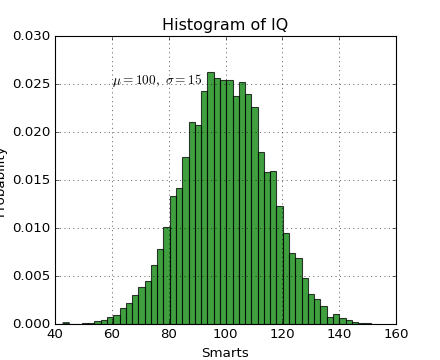
\includegraphics[width=.5\textwidth]{images/pyplot_5.png}}
  }
  \only<8>{\purple{Scatter plot}
    \prevwork{\url{http://matplotlib.org/mpl_examples/pylab_examples/scatter_demo2.py}}
    \lstinputlisting{code/pyplot_6.py}
    \vspace{-60mm}
    \flushright{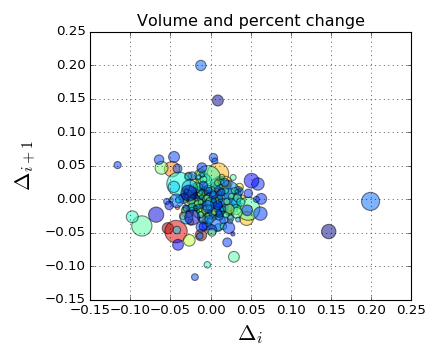
\includegraphics[width=.5\textwidth]{images/pyplot_6.png}}

  }
  \only<9>{
    \prevwork{\url{http://matplotlib.org/users/pyplot_tutorial.html}}

    \prevwork{\url{http://matplotlib.org/users/beginner.html}}
  }
\end{frame}

\talksection{Linear and Logistic Regression}

\begin{frame}
  \frametitle{Linear models}

  \only<1>{
    \textbf{Problem:}  $\{(x_i, y_i)\}$.

    Given $x$, predict $\hat y$.
  }

  \only<2>{ $x$: \textbf{explanatory} or \textbf{predictor} variable.

    $y$: \textbf{response} variable.

    \vspace{1cm}
    \purple{For some reason, we believe a linear model is a good idea.}
  }

  \only<3>{Example:
    \cimgsm{images/regression-line-1.png}
  }

  \only<4>{Example:
    \cimgsm{images/regression-line-2.png}
  }

  \only<5>{Example:
    \cimgsm{images/regression-line-3.png}
  }

  \only<6>{Example:
    \cimg{images/regression-line-4.png}
  }
\end{frame}

\begin{frame}
  \frametitle{Residuals}

  What's left over.

  \only<1>{
    \vspace{1cm}
    \begin{displaymath}
      \text{data} = \text{fit} + \text{residual}
    \end{displaymath}
  }
  \only<2>{
    \vspace{1cm}
    \begin{displaymath}
      y_i = \hat y_i + e_i
    \end{displaymath}
  }

  \only<3>{\vfill\cimg{images/residuals-1.png}}
  \only<4>{\vfill\cimg{images/residuals-2.png}}

  \only<5>{
    Goal: small residuals.

    \vspace{1cm}
    \begin{displaymath}
      \sum \mid e_i\mid
    \end{displaymath}
  }
  \only<6>{
    Goal: small residuals.

    \vspace{1cm}
    \begin{displaymath}
      \sum e_i^2
    \end{displaymath}
  }
\end{frame}

\begin{frame}
  \frametitle{Outliers}

  \only<1>{
    \vfill
    \cimghh{images/outliers-1.png}
    \cnote{
      There is one outlier far from the other points, though it only
      appears to slightly influence the line.
    }
  }

  \only<2>{
    \vfill
    \cimghh{images/outliers-2.png}
    \cnote{There is one outlier on the right, though it is quite close
      to the least squares line, which suggests it wasn’t very influential.
    }
  }

  \only<3>{
    \vfill
    \cimghh{images/outliers-3.png}
    \cnote{There is one point far away from the cloud, and this outlier appears to pull the
      least squares line up on the right; examine how the line around the primary
      cloud doesn’t appear to fit very well.
    }
  }

  \only<4>{
    \vfill
    \cimghh{images/outliers-4.png}
    \cnote{There is a primary cloud and then a small secondary cloud of four outliers. The
      secondary cloud appears to be influencing the line somewhat strongly, making
      the least square line fit poorly almost everywhere. There might be an interesting
      explanation for the dual clouds, which is something that could be investigated.
    }
  }

  \only<5>{
    \vfill
    \cimghh{images/outliers-5.png}
    \cnote{There is no obvious trend in the main cloud of points and the outlier on the
      right appears to largely control the slope of the least squares line.
    }
  }

  \only<6>{
    \vfill
    \cimghh{images/outliers-6.png}
    \cnote{There is one outlier far from the cloud, however, it falls quite close to the least
      squares line and does not appear to be very influential.
    }
  }

  \only<7>{
    \vfill\centerline{\huge Don't ignore outliers.}
  }

  \only<8>{
    \vfill
    \cimg{images/outliers-important.png}
  }
\end{frame}

\begin{frame}{Underfitting, overfitting}
  \cimg{images/under-overfitting.png}
\end{frame}

\begin{frame}
  \frametitle{Correlation}

  \only<1>{\vfill\cimgg{images/correlations-1.png}}
  \only<2>{\vfill\cimg{images/correlations-2.png}}
  \only<3>{Anscombe's Quartet

    \cimghh{images/anscombe_quartet.png}
  }
\end{frame}

\begin{frame}
  \frametitle{Hypothesis (model)}
  \begin{mphrase}
    h_\theta(x) = \theta_0 + \theta_1 x
  \end{mphrase}
\end{frame}

\begin{frame}
  \frametitle{Cost function}
  \begin{mphrase}
    J(\theta_0, \theta_1) = \frac{1}{2m} \sum_{i=1}^m (h_\theta(x_i) - y_i)^2
  \end{mphrase}
\end{frame}

\begin{frame}
  \frametitle{Gradient descent}

  \begin{mphrase}
      \begin{dcases}
        \theta_0 & \leftarrow\, \theta_0 - \alpha
        \frac{\partial}{\partial\theta_0}\, J(\theta_0, \theta_1)\\[2mm]
%
        \theta_1 & \leftarrow\, \theta_1 - \alpha
        \frac{\partial}{\partial\theta_1}\, J(\theta_0, \theta_1)
      \end{dcases}
  \end{mphrase}
\end{frame}

\begin{frame}
  \frametitle{Gradient descent}

  \begin{mphrase}
    \begin{dcases}
      \theta_0 & \leftarrow \, \theta_0 -
                 \frac{\alpha}{m} \sum_{i=1}^m (h_\theta(x_i) - y_i)
                 \\[2mm]
%
      \theta_1 & \leftarrow \, \theta_1 -
                 \frac{\alpha}{m} \sum_{i=1}^m (h_\theta(x_i) - y_i)
    \end{dcases}
  \end{mphrase}
\end{frame}

\begin{frame}
  \cimgh{images/parameter-space.png}
\end{frame}

\begin{frame}
  \frametitle{Hypothesis again}

  \begin{bphrase}
    \begin{align*}
      h_\theta(x) & = \theta_0 + \theta_1 x_1 \\[2mm]
      & = \theta_0 + \sum_{i=1}^1 \theta_i x_i \\[2mm]
      & = [\theta_0, \theta_1]
        \begin{bmatrix}
          x_0\\ x_1
        \end{bmatrix} \\[2mm]
      & = \theta^T x
    \end{align*}
  \end{bphrase}
\end{frame}

\begin{frame}
  \frametitle{Hypothesis (multiple regression)}

  \begin{bphrase}
    \begin{align*}
      h_\theta(x) & = \theta_0 + \sum_{i=1}^n \theta_i x_i \\[2mm]
      & = [\theta_0, \cdots, \theta_n]
        \begin{bmatrix}
          x_0\\ x_1 \\ \vdots \\ x_n
        \end{bmatrix} \\[2mm]
      & = \theta^T x
    \end{align*}
  \end{bphrase}
\end{frame}

\begin{frame}
  \frametitle{Hypothesis (multiple regression)}

  \begin{bphrase}
    \begin{align*}
      h_\theta(x) & = \theta^T x \\[2mm]
      & = \theta^T x^{(1)}
    \end{align*}
  \end{bphrase}
\end{frame}

\begin{frame}
  \frametitle{Hypothesis (multiple regression)}

  \begin{mphrase}
    X =
    \begin{bmatrix}
      \vline & \vline & \cdots & \vline \\
      x^{(1)} & x^{(2)} & \cdots & x^{(m)} \\
      \vline & \vline & \cdots & \vline \\
    \end{bmatrix} =
    \begin{bmatrix}
      x_0^{(1)} & x_0^{(2)} & \cdots & x_0^{(m)} \\[2mm]
      x_1^{(1)} & x_1^{(2)} & \cdots & x_1^{(m)} \\
      \vdots & \vdots & \ddots & \vdots \\
      x_n^{(1)} & x_n^{(2)} & \cdots & x_n^{(m)} \\
    \end{bmatrix}
  \end{mphrase}
\end{frame}

\begin{frame}
  \frametitle{Hypothesis (multiple regression)}

  \begin{bphrase}
    \begin{align*}
      h_\theta(X) & = \theta^T X \\[2mm]
      & =
        \begin{bmatrix}
          h_0(x^{(1)}), h_0(x^{(2)}), \cdots, h_0(x^{(m)})
        \end{bmatrix} \\
                  & = \theta^T X
    \end{align*}
  \end{bphrase}
\end{frame}

\begin{frame}
  \frametitle{Hypothesis (multiple regression)}

  \sphrase{or $X\theta$ if row vectors\ldots}
\end{frame}

\begin{frame}
  \frametitle{Cost function (multiple regression)}

  \begin{bphrase}
    \begin{align*}
      J(\theta) & = \frac{1}{2m} \sum_{i=1}^m
                  \left(h_{\theta}(x^{(i)}) - y^{(i)}\right)^2 \\
      &= \frac{1}{2m} (X\theta - Y)^T (X\theta - Y)
    \end{align*}
  \end{bphrase}
\end{frame}

\begin{frame}
  \frametitle{Gradient descent (multiple regression)}

  \begin{bphrase}
    \begin{align*}
      \theta_j & \leftarrow\, \theta_j - \frac{\alpha}{m} \sum_{i=1}^m
                 \left(h_{\theta}(x^{(i)}) - y^{(i)}\right) \cdot x_j^{(i)} \\
    \end{align*}
    \centerline{for $j=1, \cdots, n$}
  \end{bphrase}
\end{frame}

\begin{frame}
  \frametitle{Gradient descent (multiple regression)}

  \begin{bphrase}
    \begin{align*}
      \theta & \leftarrow\, \theta - \nabla J(\theta)
    \end{align*}

    \begin{displaymath}
      \mbox{where } \nabla =
      \begin{bmatrix}
        \frac{\partial}{\partial\theta_0} \\[2mm]
        \frac{\partial}{\partial\theta_1} \\[2mm]
        \vdots\\[2mm]
        \frac{\partial}{\partial\theta_n} \\
      \end{bmatrix}
    \end{displaymath}
  \end{bphrase}
\end{frame}

%%%%%%%%%%%%%%%%%%%%%%%%%%%%%%%%%%%%%%%%%%%%%%%%%%%%%%%%%%%%%%%%%%%%%%
%\talksection{Break}

\begin{frame}
  \frametitle{Linear regression}
  \begin{bphrase}
    \begin{itemize}
    \item Continuous output
    \item Normal residues
    \item Predict $\hat{y}$ for $x$ given $\{(x_i, y_i)\}$
    \end{itemize}
  \end{bphrase}
\end{frame}

\begin{frame}
  \frametitle{Logistic regression}
  \begin{bphrase}
    \begin{itemize}
    \item Binary output
    \item Classification
    \end{itemize}
  \end{bphrase}
\end{frame}

\begin{frame}
  \frametitle{Logistic regression}
  \begin{itemize}
  \item Have: continuous and discrete inputs
  \item Want: class (0 or 1)
  \end{itemize}
\end{frame}

\begin{frame}
  \frametitle{Probabilistic inspiration}
  \only<1>{
    \sphrase{{$h_\theta(x) = .75$} $\iff$ {event has 75\% of being true}}
  }
  \only<2>{
    \sphrase{$h_\theta(x) = \Pr(y=1\mid x; \theta)$ = 0.75}
  }
  \only<3>{
    \sphrase{So this must be true:}

    \sphrase{$\Pr(y=0\mid x; \theta) + \Pr(y=1\mid x; \theta)$ = 1}
  }
  \only<4>{
    \sphrase{Set $y=1 \iff h_\theta(x) = \Pr(y=1\mid x; \theta) > \frac{1}{2}$}
  }
  \only<5>{
    Math review:
    \begin{itemize}
    \item $z=(\theta^T x)$
    \item $\theta^T x \ge 0 \iff h_\theta \ge 0.5$
    \item $\theta^T x \ge 0 \iff $ predict $y=1$
    \end{itemize}

    }

\end{frame}

\begin{frame}{Logistic Regression}
  \only<1>{\cimg{images/logreg.png}}%
  \only<2>{\cimgh{images/logreg2.png}}
\end{frame}

\begin{frame}[t]
  \frametitle{Logistic (sigmoid, logit) function}
  \vspace{2cm}
  \begin{mphrase}
    g(z) = \frac{1}{1+e^{-z}}
  \end{mphrase}

  \only<2>{
    \vspace{8mm}
    Exercise: plot this}
\end{frame}

\begin{frame}[t]
  \frametitle{Cost function in logistic regression}
  \vspace{1cm}

  \only<1-3>{
    In linear regression, we had

    \begin{displaymath}
      \only<1>{J(\theta) = \frac{1}{2m} \sum_{i=1}^m (h_\theta(x^{(i)}) - y^{(i)})^2}
      \only<2>{J(\theta) = \frac{1}{2m} \sum_{i=1}^m (h_\theta(x) - y)^2}
      \only<3>{J(\theta) = \frac{1}{2m} \sum_{i=1}^m \mbox{Cost}(h_\theta(x), y)}
    \end{displaymath}
  }
  \only<4-7>{
    Here's a convex cost function:

    \begin{displaymath}
      \mbox{Cost}(h_\theta(x), y) = \begin{cases}
        -\log(h_\theta(x)) & \mbox{if } y = 1 \\[2mm]
        -\log(1-h_\theta(x)) & \mbox{if } y = 0
      \end{cases}
    \end{displaymath}

    \only<5-7>{\vspace{1cm}}
    \only<5>{
      \blue{Exercise: Plot this (cost vs $y$).}
    }
    \only<6>{
      \begin{displaymath}
        J(\theta) = \frac{1}{2m} \sum_{i=1}^m \mbox{Cost}(h_\theta(x), y)
      \end{displaymath}
    }
    \only<7>{
      \begin{displaymath}
        J(\theta) = y\cdot \log(h_\theta(x)) + (1-y) \cdot \log(1-h_\theta(x))
      \end{displaymath}
    }
  }
\end{frame}

\begin{frame}
  \frametitle{Gradient descent}
  \begin{bphrase}
    \begin{align*}
      \theta_j & \leftarrow\, \theta_j - \frac{\alpha}{m} \sum_{i=1}^m
                 \left(h_{\theta}(x^{(i)}) - y^{(i)}\right) \cdot x_j^{(i)} \\
    \end{align*}
    \centerline{for $j=1, \cdots, n$}
  \end{bphrase}
\end{frame}

\begin{frame}
  \only<1>{\phrase{null hypothesis}}
  \only<2>{\phrase{true positive, true negative}
    \vspace{1cm}
    \phrase{false positive, false negative}}
  \only<3>{\phrase{type I error}
  \centerline{(incorrect rejection of null hypothesis)}
    \vspace{1cm}
    \phrase{type II error}
    \centerline{(failure to reject null hypothesis)}}
  \only<4>{\phrase{sensitivity}\centerline{100\% sensitivity = no false negatives}}
  \only<5>{\phrase{specificity}\centerline{100\% specificity = no false positives}}
\end{frame}

\begin{frame}
  \frametitle{Precision}
  \begin{mphrase}
    P = \frac{TP}{TP + FP}
  \end{mphrase}
\end{frame}

\begin{frame}
  \frametitle{Recall}
  \begin{mphrase}
    R = \frac{TP}{TP + FN}
  \end{mphrase}
\end{frame}

\begin{frame}
  \frametitle{F1 score}
  \begin{mphrase}
    F1 = \frac{\text{precision}\cdot\text{recall}}{\text{precision} + \text{recall}}
  \end{mphrase}
\end{frame}

\begin{frame}
  \frametitle{Non-linear decision boundaries}
  \only<1> {
    \cimggg{images/non-linear-boundary.png}
    \sphrase{$h_\theta(x)) = g(\theta_0 + \theta_1 x_1 + \theta_2 x_2 + \theta_3 x_1^2 + \theta_4 x_2^2$}

    \vfill
    \prevwork{Andrew Ng}
  }
  \only<2> {
    \sphrase{OvA = OvR}
    \vspace{1cm}
    \sphrase{OvO}
  }
  \only<3> {
    \sphrase{One vs All = One vs Rest}
    \vspace{1cm}
    \sphrase{One vs One}
  }
\end{frame}

\begin{frame}
  \frametitle{One vs Rest, One vs One}
  \only<1>{
    \begin{itemize}
    \item OvR (OvA): compute $k$ classifiers
    \item OvO: compute $k(k-1)/2$ classifiers
    \end{itemize}

    The missing point: the classifiers give scores, not just in/out answers.
  }
  \only<2>{
    One vs Rest:

    Accept the judgement of the classifier with the highest score.
  }
  \only<3>{
    One vs One:

    Classifiers vote.  Accept the class that gets the most votes.
  }
  \only<3>{
    Advantage:  Reduces multi-class classification to single-class classification.

    Disadvantage:  Classifier scores aren't necessarily comparable.  For example, classes
    may have very different numbers of members.
  }
\end{frame}

\begin{frame}
  \frametitle{Hyperparameters}
  \only<1>{
    \begin{itemize}
    \item The word hyperparameter is not well-defined.
    \item In most contexts, it is the parameters of the underlying distribution
    \item In training, we learn the parameters of the model
    \item We choose the hyperparameters to govern the training
    \item So we may want to experiment to learn the distribution
      parameters that best optimise our learned model's performance
    \end{itemize}
  }
\end{frame}

\begin{frame}
  \frametitle{Testing}
  \begin{itemize}
  \item Set aside (partition) data for testing (e.g., 70\% / 30\%)
  \item Learn on training set, test on testing set
  \item When searching hyperparameters, set aside again (e.g., 60\% / 20\% / 20\%)
  \end{itemize}
\end{frame}

%%%%%%%%%%%%%%%%%%%%%%%%%%%%%%%%%%%%%%%%%%%%%%%%%%%%%%%%%%%%%%%%%%%%%%

\talksection{Support Vector Machines}

\begin{frame}
  \frametitle{The simple explanation}
  \only<1>{
    \cimghh{images/zDBbD.png}
  }
  \only<2>{
    \cimghh{images/aLZlG.png}
  }
  \only<3>{
    \cimghh{images/kxWgh.png}
  }
  \only<4>{
    \cimghh{images/ePy4V.png}
  }
  \only<5>{
    \cimghh{images/BWYYZ.png}
  }
  \only<6>{
    \cimghh{images/R9967.png}
  }
  \only<7>{
    \cimghh{images/WuxyO.png}
  }
  \only<8>{
    \cimghh{images/gWdPX.png}
  }
  \prevwork{\url{copperking@reddit}}
  % https://www.reddit.com/r/MachineLearning/comments/15zrpp/please_explain_support_vector_machines_svm_like_i
\end{frame}

\begin{frame}
  \vphrase{video time}
\end{frame}


%%%%%%%%%%%%%%%%%%%%%%%%%%%%%%%%%%%%%%%%%%%%%%%%%%%%%%%%%%%%%%%%%%%%%%

\talksectionT{CART}{Classification and Regression Trees}

\begin{frame}{$kd$-tree}
  \only<1>{
    \cimgh{images/370px-Kdtree_2d.png}
  }
  \only<2>{
    \cimgg{images/kd-tree-1.png}
  }
\end{frame}

\begin{frame}{Random subspace methods}
  Draw $k$ hyperplanes at random.
  \begin{itemize}
  \item With text, dot product, so random planes through origin
  \item With nearly everything else, random planes period
  \end{itemize}

  Result: $\log(n)$ search time
\end{frame}

\begin{frame}
  \frametitle{Decision Trees}
  \only<1>{
    Variations
    \begin{itemize}
    \item Classification tree
    \item Regression tree
    \end{itemize}
    \bigskip
    CART = classification and regression trees
  }
  \only<2>{
    % https://www.pexels.com/photo/nature-bird-australia-owl-105810/
    % https://static.pexels.com/photos/105810/pexels-photo-105810.jpeg
    % CC0 license
    \phrase{What can go wrong?}
  }
  \only<3>{
    Ensemble methods
    \begin{itemize}
    \item Bagging
    \item Random forest
    \item \gray{Boosted trees \textit{ (gradient boosted trees)}}
    \item \gray{Rotation forest}
    \end{itemize}
  }
\end{frame}

\begin{frame}
  \frametitle{Boostrap aggregating = bagging}
  \only<1>{\phrase{Boostrap}

    A family of statistical methods using sampling with replacement.

    (Also: an example of an ensemble method.)
  }
  \only<2>{
    \begin{itemize}
    \item Increase stability
    \item Increase accuracy
    \item Reduce variance
    \item Avoid overfitting
    \end{itemize}
    A type of model averaging (ensemble method).
  }
  \only<3-4>{
    \begin{itemize}
    \item Training set $D$ of size $n$
    \item Sample $D$ \textit{with replacement} to create $D_1, \ldots, D_k$ of size $n$
    \item Expect $1-1/e \approx 63.2\%$ repeats
    \end{itemize}
  }
  \only<4>{
    \begin{itemize}
    \item Train $k$ models
    \item Average (regression) or vote (classification)
    \end{itemize}
  }
  \only<5>{
    Do not confuse with
    \begin{itemize}
    \item Boosting (and AdaBoost)
    \item Boostrap (statistics)
    \item Cross validation
    \end{itemize}
  }
\end{frame}

\begin{frame}
  \frametitle{Random subspace method}
  \only<1>{
    \phrase{attribute bagging = feature bagging}
  }
  \only<2>{
    \blue{Bagging (bootstrap aggregation)} = resampling to create more
    data sets, train models on different samples

    \blue{Attribute bagging} = project to create more data sets, train
    models on different samples
  }
\end{frame}

\begin{frame}
  \frametitle{Random forests}
  \only<1>{
    \vspace{1cm}
    \centerline{Combine \blue{bagging} with \blue{random subspace method}}
  }
\end{frame}


%%%%%%%%%%%%%%%%%%%%%%%%%%%%%%%%%%%%%%%%%%%%%%%%%%%%%%%%%%%%%%%%%%%%%%


\talksection{Topic: Images}

\begin{frame}{Images}
  \only<1>{
    \phrase{Signal processing}

    \vspace{1cm}
    \centerline{in 2 or 3 dimensions}
  }
  \only<2>{
    Details that can matter:
    \begin{itemize}
    \item Illumination
    \item White balance
    \item Resolution
    \item Camera settings (e.g., depth of field)
    \item Sensor noise
    \item Compression technology
    \end{itemize}
  }
  \only<3>{
    Challenges:
    \begin{itemize}
    \item Segmentation
    \item Area of interest detection
    \item Perspective shifting
    \end{itemize}
  }
  \only<4>{
    Applications:
    \begin{itemize}
    \item Agriculture: fruit ripening, automated harvesting
    \item Security: detecting specific people
    \item Security: detecting accidents (e.g., falls)
    \item Art: counterfeit detection
    \item Medicine: assisted surgery
    \item Image search
    \end{itemize}
  }
  \only<5>{
    Image search (at first):
    \begin{itemize}
    \item Texture
    \item Colour
    \item Shape, simple objects
    \end{itemize}
  }
\end{frame}

\begin{frame}
  \cimgh{images/word2vec-1.png}
\end{frame}

\begin{frame}
  \cimghh{images/word2vec-2.png}
  \prevwork{Eddie Bell @ Lyst}
\end{frame}


%%%%%%%%%%%%%%%%%%%%%%%%%%%%%%%%%%%%%%%%%%%%%%%%%%%%%%%%%%%%%%%%%%%%%%


\talksection{PCA}

\begin{frame}
  \phrase{Principle component analysis}

  \sphrase{Analyse en composantes principales}
\end{frame}

\begin{frame}
  \frametitle{Motivation}
  \phrase{Remember the Curse of Dimensionality?}
\end{frame}

\begin{frame}[t]
  \frametitle{Principle}

  \vspace{1cm}
  \begin{itemize}
  \item Linear transformations have axes
  \item Find them (eigenvectors of the covariance matrix)
  \item Pick the biggest ones
  \end{itemize}

  \vspace{5mm}
  \only<2>{\phrase{Fitting an $n$-dimensional ellipsoid to the data}}
\end{frame}

\begin{frame}
  \frametitle{Uses}
  \begin{itemize}
  \item Exploratory data analysis
  \item Compression
  \end{itemize}
\end{frame}

\begin{frame}
  \frametitle{Also known as}
  \begin{itemize}
  \item Discrete Kosambi-Karhunen–Loève transform (KLT) (signal processing)
  \item Hotelling transform (multivariate quality control)
  \item Proper orthogonal decomposition (POD) (ME)
  \item Singular value decomposition (SVD), Eigenvalue decomposition (EVD) (linear algebra)
  \item Etc.
  \end{itemize}
\end{frame}

\begin{frame}
  \frametitle{History}
  \begin{itemize}
  \item Invented by Karl Pearson in 1901
  \item Invented (again) and named by Harold Hotelling in 1930's
  \item Also known as\dots
  \end{itemize}
\end{frame}

\begin{frame}
  \frametitle{Also known as}

  \begin{itemize}
  \item It's a long list, every field uses a different name\dots
  \end{itemize}
\end{frame}

\begin{frame}{In addition to PCA\dots}
  There are newer methods that are sometimes better.

  \begin{itemize}
  \item Sometimes they are faster.
  \item Sometimes the projection makes more sense.
  \end{itemize}

  $t$-SNE is the most common you'll encounter.
\end{frame}


\talksection{Topic: Face Recognition}

\begin{frame}
  \frametitle{Eigenfaces}
  \only<1>{
    \begin{itemize}
    \item Sirovich and Kirby (1987)
    \item Turk and Pentland (1991)
    \end{itemize}
    \vfill
    \prevwork{Turk, Matthew A and Pentland, Alex P. Face recognition
      using eigenfaces. Computer Vision and Pattern Recognition,
      1991. Proceedings {CVPR'91.}, {IEEE} Computer Society Conference
      on 1991.}
  }
  \only<2>{ Want: a low-dimensional representation of a face

    Plan: cluster simplified faces
  }
  \only<3>{
    Viewed as compression:
    \begin{itemize}
    \item Use PCA on face images to form a set of basis features
    \item Use eigenpictures to reconstruct original faces
    \end{itemize}
  }
  \only<4>{
    \cimghh{images/eigenface-reconstruction-opencv.png}
  }
\end{frame}

\begin{frame}
  \frametitle{Eigenfaces algorithm}

  \only<1>{
    Let $X=\{x_1, x_2, \dotsc, x_n\}$ be a random vector with observations $x_i\in\mathbb{R}^d$.

    Compute

    \begin{displaymath}
      \mu=\frac{1}{n} \sum_{i=1}^n x_i
    \end{displaymath}

    \vfill
    \prevwork{OpenCV}
  }
  \only<2>{
    Compute the covariance matrix $S$:

    \begin{align*}
      S_{i,j} & = \cov(x_i, x_j) \\
              & = \E[(x_i-\mu_i)(x_j-\mu_j)^T] \\[7mm]
      S & = (S_{i,j})
    \end{align*}
  }
  \only<3-4>{
    Compute the eigenvectors of $S$:

    \begin{displaymath}
      Sv_i = \lambda_i v_i \qquad i=1,2,\dotsc, n
    \end{displaymath}

    Sort the eigenvectors in decreasing order.

    We want the $k$ principal components, so take the first $k$.

    \only<4>{\blue{This is PCA.}}
  }
  \only<5>{
    The $k$ principal components of the observed vector $x$ are then given by

    \begin{displaymath}
      y=W^T(x-\mu)
    \end{displaymath}

    where
    \begin{displaymath}
      W = \begin{bmatrix}
        \vline & \vline & & \vline \\
        v_1& v_2 & \cdots & v_k \\
        \vline & \vline & & \vline
      \end{bmatrix}
    \end{displaymath}
  }
  \only<6>{
    The reconstruction from the PCA basis is then

    \begin{displaymath}
      x = Wy + \mu
    \end{displaymath}
  }
  \only<7>{
    So the plan is this:
    \begin{itemize}
    \item Project all training samples in the PCA subspace
    \item Project the query into the PCA subspace
    \item Find the nearest neighbour to the projected query image among
      the projected training images
    \end{itemize}
  }
  \only<8>{
    \cimghh{images/eigenface-reconstruction-opencv.png}
  }
  \only<9>{
    Some advantages:
    \begin{itemize}
    \item Easy, relatively inexpensive
    \item Recognition cheaper than preprocessing
    \item Reasonably large database possible
    \end{itemize}
  }
  \only<10>{
    Some problems:
    \begin{itemize}
    \item Need controlled environment
    \item Needs straight-on view
    \item Sensitive to expression changes
    \item If lots of variance is external (e.g., lighting)\dots
    \end{itemize}
  }
\end{frame}


\talksection{Topic: Handwriting Recognition}

\begin{frame}
  \frametitle{Introduction to Handwriting Recognition}
  \only<1>{
    Choices
    \begin{itemize}
    \item Online
    \item Offlne
    \end{itemize}
  }
  \only<2>{
    Choices
    \begin{itemize}
    \item Get path information
    \item Get time data
    \item Get pressure information
    \item Only get image
    \end{itemize}
  }
  \only<3>{
    Major techniques
    \begin{itemize}
    \item Clustering (not great performance)
    \item SVM (until 2006 or so)
    \item Convolutional neural networks
    \end{itemize}
  }
\end{frame}

\talksection{Clustering}

\begin{frame}
  \frametitle{The Problem}
  Have points $d = \{d_1, \dotsc, d_n\}$.

  Have number of clusters $k$.

  \vspace{5mm}
  \textbf{Want:} an assignment of points to clusters
\end{frame}

\begin{frame}
  \cimggg{images/cluster-1.png}
\end{frame}

\begin{frame}
  \cimgh{images/cluster-2.png}
\end{frame}

\begin{frame}
  \cimg{images/cluster-3.png}
\end{frame}

\begin{frame}
  \cimg{images/cluster-4.png}
\end{frame}

\begin{frame}
  \frametitle{The Algorithm}
  \begin{enumerate}
  \item Assign points to clusters at random
  \item Repeat until stable:
  \begin{enumerate}
  \item Compute centroids of each cluster
  \item Assign points to nearest centroid
  \end{enumerate}
  \end{enumerate}
\end{frame}


\begin{frame}
  \frametitle{Cost function}
  \begin{mphrase}
    \textrm{cost} = \sum_i \sum_j \left| x_j - \mu_i \right|
  \end{mphrase}
\end{frame}

\begin{frame}
  \frametitle{Silhouette coefficient}
  \only<1-2>{
    Points $d = \{d_1, \dotsc, d_n\}$

    Clusters $K = \{c_1, \dotsc, c_k\}$.

    Cluster $c_{d_i}$ is the centroid of $d_i$.
  }

  \only<2>{
    \blue{Let $a_i$ be the average dissimilarity of $d_i$ to all
      points in its cluster.}

    \blue{Let $b_i$ be the least average dissimilarity of $d_i$ to any
      cluster other than $k_{d_i}$}
  }

  \only<3-5>{
    \begin{mphrase}
      s_i = \frac{b_i - a_i}{\max\{a_i, b_i\}}
    \end{mphrase}
  }

  \only<4-5>{
    \begin{mphrase}
      s_i = \left\{
        \begin{array}{ll}
          1 - a_i/b_i & \mbox{ if } a_i < b_i \\[2mm]
          0 & \mbox{ if } a_i = b_i \\[2mm]
          b_i / a_i - 1 & \mbox{ if } a_i > b_i
        \end{array}\right.
    \end{mphrase}
  }

  \only<5>{
    So $s_i \in [-1, 1]$
  }

  \only<6>{
    $s_i$ near 1 $\iff$ $d_i$ well clustered

    $s_i$ near 0 $\iff$ $d_i$ on the border between two clusters

    $s_i$ near -1 $\iff$ $d_i$ poorly clustered
  }

  \only<7>{
    \begin{mphrase}
      \textrm{Consider } \overline{s_i} \,\textrm{ over } i\in c_j \textrm{ for cluster } c_j
    \end{mphrase}
  }

  \only<8>{
    \begin{mphrase}
      \textrm{Consider } \overline{s_i}
    \end{mphrase}
  }
\end{frame}

\begin{frame}
  \vphrase{video time}
\end{frame}

\talksection{Topic: Anomaly Detection}

\begin{frame}
  \frametitle{Introduction to Anomaly Detection}
  \only<1>{
    \begin{itemize}
    \item Supervised
    \item Unsupervised
    \end{itemize}
  }
  \only<2>{
    Supervised anomaly detection:
    \begin{itemize}
    \item Training data: normal, abnormal
    \item Train a classifier
    \end{itemize}

    So reduced to existing problem of supervised classification.
  }
  \only<3>{
    Unsupervised anomaly detection:
    \begin{itemize}
    \item Mostly, this is clustering
    \item Increasingly, this is neural networks in advanced applications
    \end{itemize}
  }
  \only<4>{
    Applications:
    \begin{itemize}
    \item Intrusion detection (physical or electronic)
    \item Fraud detection
    \item Health monitoring (people, animals, machines)
    \end{itemize}
  }
  \only<5>{
    Techniques:
    \begin{itemize}
    \item Density: kNN, local outlier factor
    \item SVM
    \item Clustering: $k$-Means
    \end{itemize}
  }
  \only<6>{
    kNN techniques and variations
    \begin{itemize}
    \item Voronoi diagrams
    \item aNN
    \end{itemize}
  }
  \only<7>{
    LOF
    \begin{itemize}
    \item Measure average density using kNN
    \item Points with low local density are suspect outliers
    \item There is no good thresholding technique
    \end{itemize}
  }
  \only<8>{
    $k$-Means
  }
\end{frame}

\begin{frame}
  \frametitle{Examples}
  \only<1>{
    \vphrase{ping times}
  }
  \only<2>{
    \vphrase{httpd response times}
  }
  \only<3>{
    \vphrase{single/multiple host access abuse (DOS/DDOS)}
  }
  \only<4>{
    \vphrase{bank card fraud}
  }
  \only<5>{
    \vphrase{spam}
  }
\end{frame}


\talksection{Topic: Anomaly Detection (not time)}

\begin{frame}
  \frametitle{Introduction to Anomaly Detection}
  \only<1>{
    \begin{itemize}
    \item Supervised
    \item Unsupervised
    \end{itemize}
  }
  \only<2>{
    Supervised anomaly detection:
    \begin{itemize}
    \item Training data: normal, abnormal
    \item Train a classifier
    \end{itemize}

    So reduced to existing problem of supervised classification.
  }
  \only<3>{
    Unsupervised anomaly detection:
    \begin{itemize}
    \item Mostly, this is clustering
    \item Increasingly, this is neural networks in advanced applications
    \end{itemize}
  }
  \only<4>{
    Applications:
    \begin{itemize}
    \item Intrusion detection (physical or electronic)
    \item Fraud detection
    \item Health monitoring (people, animals, machines)
    \end{itemize}
  }
  \only<5>{
    Techniques:
    \begin{itemize}
    \item Density: kNN, local outlier factor
    \item SVM
    \item Clustering: $k$-Means
    \end{itemize}
  }
  \only<6>{
    kNN techniques and variations
    \begin{itemize}
    \item Voronoi diagrams
    \item aNN
    \end{itemize}
  }
  \only<7>{
    $k$-Means
  }
\end{frame}

\talksection{Local Outlier Factor}

\begin{frame}{Local Outlier Factor (LOF)}
  \only<1>{
    \begin{itemize}
    \item Measure average density using kNN
    \item Points with low local density are suspect outliers
    \item There is no good thresholding technique
    \end{itemize}
  }
  \only<2> {
    Let $a$ be an object (point) in the set of samples.

    Let $N_k(a)$ be the set of $k$ nearest neighbours to $a$.

    Define the $k$-distance from $a$:

    \begin{displaymath}
      d_k(a) = \max_{p\in N_k(A)} d(a, p)
    \end{displaymath}
  }
  \only<3> {
    Define now the reachability distance:

    \begin{displaymath}
      r_k(a, b) = \max (d_k(a), d(a, b))
    \end{displaymath}

    In otherwords, $r_k$ is the distance between two points, but is no
    less than the $k$-distance.

    So all the points in $N_k(a)$ are considered equally $r_k$ distant
    from $a$.

    \bigskip
    \purple{Math note: $r_k$ is not a true distance function.}
  }
  \only<4> {
    Define the \textit{local reachability density} of object $a$ by

    \begin{displaymath}
      \mbox{lrd}(a) = \frac{1}{\left(
          \frac{
            \sum\limits_{b\in N_k(a)} r_k(a, b)
          }
          {|N_k(A)|}
        \right)}
      =
      \left(
      \frac
      {|N_k(A)|}
      {
        \displaystyle\sum_{b\in N_k(a)} r_k(a, b)
      }
      \right)
    \end{displaymath}

    This is the (inverse of the) average reachability distance of the
    $k$ nearest neighbours.
  }
  \only<5> {
    The

    \begin{displaymath}
      \mbox{LOF}_k(a) = \left(
        \frac
        {\sum_{b\in N_k(a)} \frac{\mbox{lrd}(b)}{\mbox{lrd}(a)}}
        {|N_k(a)|}
        \right)
        =
        \left(
          \frac
          {\sum_{b\in N_k(a)} \mbox{lrd}(b)}
          {|N_k(a)|\quad \mbox{lrd}(a)}
        \right)
      \end{displaymath}

      \bigskip
      \blue{Interpretation:}
      \begin{itemize}
      \item \blue{1} indicates a point is comparable to its neighbours
      \item \blue{$<1$} indicates more densely packed than its neighbours
      \item \blue{$>1$} indicates more sparsely packed than its neighbours
      \end{itemize}

  }
  \only<6>{
    \cimghh{images/LOF-idea.png}
    \vspace{-3cm}
    \prevwork{By Chire - Own work, Public Domain,
      \url{https://commons.wikimedia.org/w/index.php?curid=10423954}}
  }
  \only<7>{
    \cimghh{images/LOF-example.png}
    \prevwork{By Chire - Own work, Public Domain,
      \url{https://commons.wikimedia.org/w/index.php?curid=10423954}}
  }
  \only<8>{
    Advantages: intuitive, often works well (e.g., intrusion detection)

    Disadvantages: fails at higher dimension (curse of
    dimensionality), hard to interpret
  }
\end{frame}


\talksection{Topic: Music}

\begin{frame}
  \cimghh{images/fourier-1.png}
  \prevwork{\url{http://www.toptal.com/algorithms/shazam-it-music-processing-fingerprinting-and-recognition}}
\end{frame}

\begin{frame}
  \cimghh{images/fourier-2.png}
  \prevwork{\url{https://www.ee.columbia.edu/~dpwe/papers/Wang03-shazam.pdf}}
\end{frame}

\begin{frame}
  \cimghh{images/fourier-hash.png}
  \prevwork{\url{https://www.ee.columbia.edu/~dpwe/papers/Wang03-shazam.pdf}}
\end{frame}


\talksection{Topic: Time Series}

\begin{frame}
  \frametitle{Introduction to time series}
  \only<1>{
    \purple{This is hard, but it depends on your goals.  And on context.}
  }
  \only<2>{
    Definition (discrete time series):

    \begin{displaymath}
      \{s_t\mid t\in\mathbb{R}^+\wedge s\in\mathbb{R}\}
    \end{displaymath}

    \purple{(though $s$ in any vector space is fine)}
  }
  \only<3>{
    Examples domains:
    \begin{itemize}
    \item Weather
    \item Economics
    \item Industry (e.g., factories)
    \item Medicine
    \item Web
    \item Biological processes
    \end{itemize}
  }
  \only<4>{
    Why?
    \begin{itemize}
    \item Predict
    \item Control
    \item Understand
    \item Describe
    \end{itemize}
  }
  \only<5>{
    Some strategies:
    \begin{itemize}
    \item Differencing:\\ \hspace{1cm}
      $y_t' = y_t - y_{t-1}$ \\[2mm]
    \item Second-order differencing: \\ \hspace{1cm}
      $y_t'' = (y_t - y_{t-1}) - (y_{t-1} - y_{t-2}) = y_t - 2y_{t-1}
      + y_{t-2}$
    \end{itemize}
  }
  \only<6>{
    Some strategies:
    \begin{itemize}
    \item Clustering
    \item Hidden Markov Models (HMM)
    \item Recurrent neural networks (RNN)
    \item Autoregressive integrated moving average (ARIMA)
      \begin{itemize}
      \item Generalisation of autoregressive moving average (ARMA)
        model
      \item Regress on series' own lag
      \end{itemize}

    \end{itemize}
  }
  \only<7>{
    One model:
    \begin{displaymath}
      s_t = g(t) + \phi_t
    \end{displaymath}

    where
    \begin{itemize}
    \item[] $g(t)$ is deterministic: signal (or trend)
    \item[] $\phi_t$ is stochastic noise
    \end{itemize}
  }
  \only<8>{
    Variation types:
    \begin{itemize}
    \item Trend ($g$)
    \item Seasonal effect ($g$)
    \item Irregular fluctuation (residuals: $\phi$)
    \end{itemize}
  }
  \only<9>{
    \cimghh{images/decomposition.png}
    \vspace{-8mm}
    \prevwork{\url{http://www.ulb.ac.be/di/map/gbonte/ftp/time_ser.pdf}}
  }
\end{frame}

\begin{frame}
  \frametitle{Introduction to time series}

  Some easy things to try

  \begin{itemize}
  \item Introduce features to break out seasonality
  \item Introduce lags as features
  \item Some domain-specific transformation
  \end{itemize}
\end{frame}


\talksection{Hidden Markov Models}

\begin{frame}
  \phrase{``simplest dynamic Bayesian network''}
\end{frame}

\begin{frame}
  \frametitle{Markov Chains}
  \only<1>{
    A \textbf{Discrete time Markov chain (DTMC)} is a random process that
    undergoes state transitions.
  }
  \only<2>{
    \begin{displaymath}
      \begin{bmatrix}
        x_{11} & x_{12} & \cdots & x_{1n} \\[2mm]
        x_{21} & x_{22} & \cdots & x_{2n} \\[2mm]
        \vdots & & \ddots & \vdots \\[2mm]
        x_{n1} & x_{n2} & \cdots & x{nn}
      \end{bmatrix}
      \begin{bmatrix}
        v^{(i)}_1 \\[2mm]
        v^{(i)}_2 \\[2mm]
        \vdots \\[2mm]
        v^{(i)}_n
      \end{bmatrix}
      =
      \begin{bmatrix}
        v^{(i+1)}_1 \\[2mm]
        v^{(i+1)}_2 \\[2mm]
        \vdots \\[2mm]
        v^{(i+1)}_n
      \end{bmatrix}
    \end{displaymath}
  }
  \only<3>{
    \begin{displaymath}
      Xv_i = v_{i+1}
    \end{displaymath}
  }
  \only<4>{
    Examples:
    \begin{itemize}
    \item Random walks
    \item Weather (first approximation in many places)
    \item Thermodynamics
    \item Queuing theory (so also telecommunications)
    \item Spam
    \end{itemize}
  }
  \only<5>{
    Properties:
    \begin{itemize}
    \item Stochastic process
    \item Memoryless (``Markov property'')
    \end{itemize}
  }
\end{frame}

\begin{frame}
  \frametitle{HMM's}
  \only<1>{
    \begin{itemize}
    \item State is not visible
    \item Output of state is visible
    \end{itemize}

    Examples: noisy sensor, medical diagnosis
  }
  \only<2>{
    What we have:\vspace{-2.5mm}
    \begin{itemize}
    \item State space $S = \{s_1, \dotsc, s_n \}$
    \item Observation space $O = \{o_1, \dotsc, o_k \}$
    \item Transition matrix $A$ of size $n\times n$
    \item Emission matrix $B$ of size $n\times k$
    \item Initial state probabilities $\pi = \{\pi_1, \dotsc, \pi_n \}$
    \item A sequence of observations $X=\{x_1, \dotsc x_T \}$
    \end{itemize}

    Here\vspace{-2.5mm}
    \begin{itemize}
    \item $y_t = i \iff $ observation at time $t$ is $o_i$
    \item $\Pr(x_1 = s_i) = \pi_i$
    \end{itemize}

    We want the sequence of states $X=\{x_1, \dotsc, x_T \}$.

  }
  \only<3>{
    Some pointers to learn more about HMM:
    \begin{itemize}
    \item Forward-Backward Algorith
    \item Viterbi Decoding
    \item Baum-Welch Algorithm
    \end{itemize}
  }
\end{frame}


\talksection{Topic: Recommendation}


\begin{frame}
  \frametitle{Definition}

  \vspace{1cm}
  \centerline{\parbox{.8\textwidth}{ Given data about a user, his
  environment, and some items of interest (\textit{training data}),
  determine items to recommend.}}

  \vspace{1cm}
  \only<2>{
    We don't have to find the $\max k$.

    It's enough to find $k$ within some $\max n$.
  }
\end{frame}

\begin{frame}
  \frametitle{Examples}
  \begin{itemize}
  \item Amazon
  \item Google News (or Le Monde)
  \item Facebook
  \item Medical testing
  \item App Store / Google Play
  \item Youtube
  \item Advertising
  \item Netflix, last.fm, Spotify, Pandora, \dots
  \item Browser (URL recommendations)
  \item Search
  \end{itemize}
  % TODO: images
\end{frame}

\begin{frame}
  \frametitle{Client Value Proposition}
  \begin{itemize}
  \item Find opportunities
  \item Reduce choice
  \item Explore options
  \item Discover long tails
  \item Recreation
  \end{itemize}
\end{frame}

\begin{frame}
  \frametitle{Provider Value Proposition}

  \begin{itemize}
  \item Offer a unique or additional service (beyond competitors)
  \item Customer trust and loyalty
  \item Increase sales, CTR, conversions
  \item Better understand customers
  \end{itemize}
\end{frame}

% ======================================================================
% Technique Overview

\begin{frame}
  \frametitle{Recommendation}

  \begin{tabular}{|p{5.7cm}|p{4cm}|}
    \hline
    \topstrut\hbox{Content-based filtering}
    \hbox{\it (filtrage basée sur le contenu)}
    &
    More things similar to what I like\bottomstrut
    \\
    \hline
    \topstrut\hbox{Collaborative filtering}
    \hbox{\it (filtrage collaboratif)}
    &
    More of what other people who like what I like like
    \bottomstrut
    \\
    \hline
    \topstrut\hbox{Knowledge-based filtering}
    \hbox{\it (filtrage basée sur connaissance)}\bottomstrut
    &
    More of what I need.\bottomstrut
    \\
    \hline
  \end{tabular}
\end{frame}

\begin{frame}[t]
  \frametitle{Content-based filtering}
  \textit{\purple{More things similar to what I like}}\\
  \textit{\red{Plus de ce qui ressemble à ce que j'aime}}

  Advantages\vspace{-2mm}
  \begin{itemize}
  \item [yes!] No need for community
  \item [yes!] Possible to compare items
  \end{itemize}

  \medskip
  Disadvantages\vspace{-2mm}
  \begin{itemize}
  \item [no] Understand content
  \item [yes] Cold start problem
  \item [no] Serendipity
  \end{itemize}
\end{frame}

\begin{frame}[t]
  \frametitle{Collaborative filtering}
  \textit{\purple{More of what other people who like what I like like}}\\
  \textit{\red{Plus de ce que d'autres qui aiment ce que j'aime aiment}}

  Advantages\vspace{-2mm}
  \begin{itemize}
  \item [yes!] No need to understand content
  \item [yes!] Serendipity
  \item [yes!] Learn market
  \end{itemize}

  \medskip
  Disadvantages\vspace{-2mm}
  \begin{itemize}
  \item [no] User feedback
  \item [yes] Cold start problem (users)
  \item [yes] Cold start problem (items)
  \end{itemize}
\end{frame}

\begin{frame}[t]
  \frametitle{Knowledge-based filtering}
  \textit{\purple{More of what I need}}\\
  \textit{\red{Plus de ce qu'il faut}}

  Advantages\vspace{-2mm}
  \begin{itemize}
  \item [yes!] Deterministic
  \item [yes!] Certainty
  \item [no!] Cold start problem
  \item [yes!] Market knowledge
  \end{itemize}

  \medskip
  Disadvantages\vspace{-2mm}
  \begin{itemize}
  \item [yes] Studies to bootstrap
  \item [yes] Static model, doesn't learn from trends
  \end{itemize}
\end{frame}


% ======================================================================
% Linear Algebra Basics

\begin{frame}[t]
  \frametitle{Utility Matrix}

  \begin{itemize}
  \item Users (utilisateurs)
  \item Items (objets)
  \end{itemize}

  \only<2->{The goal is to fill in the blanks.}

  \only<2>{
    \vspace{1cm}
    \centerline{\begin{tabular}{l|ccccc}
        & $I_1$ & $I_2$ & $I_3$ & $I_4$ & $I_5$ \\
        \hline
        $U_1$ & 1 & & & & \\
        $U_2$ & & & 1 & 1 & 1 \\
        $U_3$ & & 1 & & 1 & 1
      \end{tabular}}

    \bigskip
    \centerline{\gray{Example: books sales at Amazon.}}
  }
  \only<3>{
    \vspace{1cm}
    \centerline{\begin{tabular}{l|ccccc}
        & $I_1$ & $I_2$ & $I_3$ & $I_4$ & $I_5$ \\
        \hline
        $U_1$ & 3 & & & & \\
        $U_2$ & & & 5 & 1 & 4 \\
        $U_3$ & & 2 & & 5 & 1
      \end{tabular}}

    \bigskip
    \centerline{\gray{Example: film advice at Netflix.}}
  }

  \only<2->{
    \bigskip
    \gray{\it But thousands or millions of columns and rows.}
  }
\end{frame}

\begin{frame}
  \frametitle{Utility Matrix}

  How do we make the matrix?
  \begin{itemize}
  \item Ask users
  \item Observe users
  \end{itemize}

  That's usually expensive\dots
\end{frame}

\begin{frame}
  \frametitle{Item Profiles}

  Examples:
  \begin{itemize}
  \item Films \gray{$\qquad\Rightarrow$ ?}
  \item Books \gray{$\qquad\Rightarrow$ ?}
  \item News \gray{$\qquad\Rightarrow$ ?}
  \item Images \gray{$\qquad\Rightarrow$ ?}
  \end{itemize}

  \only<2>{\gray{ Films :}

    \gray{Content: acters, directors, year (decade, etc.), length}

    \gray{Collaborative: seen, opinion~(1--5), when seen relative to release}
  }
  \only<3>{\gray{Books:}

    \gray{Content : authers, genre, year (decade, etc.), number of pages, content (very difficult)}

    \gray{Collaborative: read, opinion~(1--5), how read}
  }
  \only<4>{\gray{News:}

    \gray{Content : source, section, TF-IDF word vectors}

    \gray{Collaborative: }
  }
  \only<5>{\gray{Images :}

    \gray{Content:}

    \gray{Collaborative:}
  }

  \only<6>{

    \gray{Also: user profile, user behavior}
  }

\end{frame}

\begin{frame}
  \frametitle{Mathematics}

  \vspace{1cm}
  \centerline{Vectors}

  \vspace{1cm}
  \centerline{Similarity}
\end{frame}

\begin{frame}
  \frametitle{Similarity : Jaccard Index}

  \only<1>{\green{or: \textit{Indice de Jaccard}, \textit{Jaccard similarity coefficient}}}

  \vspace{1cm}
  Similarity:
  \begin{displaymath}
    J(A,B) = \frac{|A\cap B|}{|A\cup B|}
  \end{displaymath}

  \only<2>{
    Distance:
    \begin{displaymath}
      J_{\delta}(A,B) = 1 - J(A,B)
    \end{displaymath}
  }
\end{frame}

\begin{frame}
  \frametitle{cosine similarity}

  \only<1>{\green{or: \textit{mesure cosinus}, \textit{Similarité cosinus}}}

  \vspace{1cm}
  Similarity:
  \only<1>{
    \begin{displaymath}
      \cos \theta = \frac{A\cdot B}{\parallel A\parallel \parallel B\parallel}
    \end{displaymath}
  }
  \only<2->{
    \begin{displaymath}
      S_C(A,B) = \frac{A\cdot B}{\parallel A\parallel \parallel B\parallel}
    \end{displaymath}
  }

  \only<3->{
    Distance:
    \begin{displaymath}
      D_C(A,B) = 1-S_C(A,B)
    \end{displaymath}
  }

  \only<4>{
    \gray{We only consider non-empty components in the vector.}
  }
\end{frame}

\begin{frame}
  \frametitle{Texts: TF-IDF}

  \begin{itemize}
  \item Vectors of word frequencies
  \item Frequency $\centernot\implies$ significance
  \item<2> Term Frequency - Inverse Document Frequency
  \end{itemize}
\end{frame}

\begin{frame}
  \frametitle{Texts: TF-IDF}

  \blue{
    \begin{displaymath}
      TF_{ij} = \frac{f_{ij}}{\max_k f_{kj}} \qquad\qquad
      IDF_I = \log_2\left( \frac{N}{n_i} \right)
    \end{displaymath}
  }
  \blue{
    \begin{displaymath}
      TF\mbox{-}IDF_{ij} = TF_{ij} \cdot IDF_i
    \end{displaymath}
  }
  with :
  \begin{align*}
    f_{ij} &= \mbox{frequency of word $i$ in document $j$} \\
    N &= \mbox{number of documents}\\
    n_i &= \mbox{number of documents in which we find word $i$}
  \end{align*}

  \only<2->{
    IDF is a mesure of how much information a word carries

    TF-IDF tells us which words best characterise a document
  }

  \only<3>{
    \vspace{-3mm}
    \gray{Variation: boolean, log, stop word filtering}
  }
\end{frame}


% ======================================================================
% Item-Item Filters

\begin{frame}
  \frametitle{Content-Based Filtering}

  \vspace{1cm}

  \vspace{15mm} % A fragile hack.
  \centerline{\fcolorbox{blue}{white}{\hspace{55mm}\rule{0pt}{1.45ex}}}
  \vspace{-15mm}

  \centerline{\begin{tabular}{l|ccccc}
      & $I_1$ & $I_2$ & $I_3$ & $I_4$ & $I_5$ \\
      \hline
      $U_1$ & 3 & & & & \\
      $U_2$ & & & 5 & 1 & 4 \\
      $U_3$ & & 2 & & 5 & 1
    \end{tabular}}

  \vspace{1cm}
  \centerline{\purple{More things similar to what I like}}

  \centerline{\textit{\red{Plus de ce qui ressemble à ce que j'aime}}}

  \only<2>{
    \vspace{1cm} \gray{Then, we can cluster (\textit{regroupement},
      \textit{partitionnement de données}), etc.}  }
\end{frame}

\begin{frame}
  \frametitle{Content-Based Filtering}

  % TODO: Define this
  % TODO: Item-Item Filters

  Based on item profiles
  \begin{itemize}
  \item More stable (in principle)
  \item $O(n^2)$ (but often less, items often aren't categorised together)
  \item Can reduce to threshold
  \item Can pre-calculate, queries become faster
  \end{itemize}
\end{frame}


% ======================================================================
% Collaborative Filters

\begin{frame}
  \frametitle{Collaborative Filtering}

  \vspace{1cm}
  \centerline{\begin{tabular}{l|ccccc}
      & $I_1$ & $I_2$ & $I_3$ & $I_4$ & $I_5$ \\
      \hline
      $U_1$ & 3 & & \fcolorbox{blue}{white}{4} & \fcolorbox{blue}{white}{2} & \\
      \fcolorbox{blue}{white}{$U_2$} & & & 5 & 1 & 4 \\
      $U_3$ & & 2 & & 5 & 1
    \end{tabular}}

  \vspace{1cm}
  \centerline{\purple{More of what other people who like what I like like}}

  \centerline{\textit{\red{Plus de ce que d'autres qui aiment ce que j'aime aiment}}}
\end{frame}

\begin{frame}
  \frametitle{Collaborative Filtering}

  \vspace{1cm}

  \vspace{15mm} % A fragile hack.
  \centerline{\fcolorbox{blue}{white}{\hspace{55mm}\rule{0pt}{1.45ex}}}
  \vspace{-15mm}

  \centerline{\begin{tabular}{l|ccccc}
      & $I_1$ & $I_2$ & $I_3$ & $I_4$ & $I_5$ \\
      \hline
      $U_1$ & 3 & & & & \\
      $U_2$ & & & 5 & 1 & 4 \\
      $U_3$ & & 2 & & 5 & 1
    \end{tabular}}

  \vspace{1cm}
  \centerline{User profile}
\end{frame}

\begin{frame}
  \frametitle{Collaborative Filtering}

  \vspace{1cm}

  % A fragile hack.
  \vspace{19mm}
  \centerline{\hspace{8mm}\fcolorbox{blue}{white}{\hbox to 10pt{\vbox to 19mm{}}}}
  \vspace{-20mm}

  \centerline{\begin{tabular}{l|ccccc}
      & $I_1$ & $I_2$ & $I_3$ & $I_4$ & $I_5$ \\
      \hline
      $U_1$ & 3 & & 4 & 2 & \\
      $U_2$ & & & 5 & 1 & 4 \\
      $U_3$ & & 2 & & 5 & 1
    \end{tabular}}

  \vspace{1cm}
  \centerline{Item profile}
\end{frame}

\begin{frame}
  \frametitle{Utility Matrix Symmetry}

  \begin{itemize}
  \item Propose items based on users
  \item Propose users based on items
  \end{itemize}

  \only<2-3>{But remember: \blue{2 items being similar
      $\,\centernot\equiv\,$ 2 users similar.}
  }
  \only<3>{\vspace{1cm}

    \purple{Thought experiment: consider comparing people vs comparing objects.}
  }

  \only<4>{
      To estimate $m_{u,i}$,
      \begin{itemize}
      \item Find $k$ users like $U_u$
      \item Find $k$ items like $I_i$
      \end{itemize}
    }
\end{frame}

\begin{frame}
  \frametitle{Utility Matrix : Estimate $m_{u,i}$}

  \vspace{1cm}
  \centerline{\begin{tabular}{l|ccccc}
      & $I_1$ & $I_2$ & $I_3$ & $I_4$ & $I_5$ \\
      \hline
      $U_1$ & 3 & & 4 & 2 & \fcolorbox{blue}{white}{\rule{0pt}{.9ex}\ }\\
      $U_2$ & & & 5 & 1 & 4 \\
      $U_3$ & & 2 & & 2 & 3
    \end{tabular}}

  \bigskip
  \begin{itemize}
  \item Find $k$ users like $U_u$, take $\frac{1}{k}
    \sum_{j=1}^k m_{u_j,i}$
  \item Find $k$ items like $I_i$, take $\frac{1}{k}
    \sum_{j=1}^k m_{u,i_j}$
  \end{itemize}

  \only<2>{
    \gray{We have to compute the entire line (or the part which is likely to be important)}
  }
  \only<3>{
    \gray{Once we've computed $U_u$, the other $k$ users lets us take a shortcut.}
  }
  \only<4>{
    \gray{For $I_i$, we have to compute most of the $I_j$ before we
      can fill in a single line.  But item-item filters are often
      more reliable.}
  }
  \only<5>{
    \gray{In any case, we can mostly precompute in advance.}
  }
\end{frame}

\begin{frame}
  \frametitle{Utility Matrix}

  The matrix is sparse.

  $\implies$ clustering $\implies$ reduced matrix

  \only<2>{\gray{Estimate on the reduced matrix, then take items and
      users as representative for the cluster.}}
\end{frame}


% ======================================================================
% Amazon's Item-Item Filter

\begin{frame}
  \frametitle{Amazon : Item-to-Item Collaborative Filtering}

  Observations :
  \vspace{1cm}

  \centerline{
    \only<1>{\blue{Clustering is expensive, reduces quality}}
    \only<2>{\blue{Dimension reduction reduces quality}}
    \only<3>{\blue{Users interact with very few items}}
    \only<4>{\blue{Rapid response desirable}}
  }
\end{frame}

\begin{frame}
  \frametitle{Amazon : Item-to-Item Collaborative Filtering}

  Scales independent of the number of users or of items
  \begin{itemize}
  \item Online
  \item Offline
  \end{itemize}

  \bigskip
  \gray{G.~Linden, B.~Smith, J.~York, \textit{Amazon.com
      Recommendations: Item-to-Item Collaborative Filtering}, Internet
  Computing (7, 1), 22 Jan 2003.}

\end{frame}

\begin{frame}
  \frametitle{Amazon : Item-to-Item Collaborative Filtering}
  Offline (Precomputation)

  \DontPrintSemicolon
  \begin{algorithm}[H]
    \For{each item $I_1$ to sell}{
      \For{each user $C$ who has purchased $I_1$}{
        \For{each item $I_2$ bought by $C$}{
          $(I_1,I_2)$++\;
        }
      }
      \For{each item $I_2$}{
        $S_{I_1,I_2} \gets S(I_1,I_2)$\;
      }
    }
  \end{algorithm}
\end{frame}


% ======================================================================
% Slope One

\begin{frame}
  \frametitle{Slope One}

  \vspace{1cm}
  Linear regression on user opinions (ratings)
  \vspace{1cm}

  \gray{Daniel Lemire and Anna Maclachlan, \textit{Slope One
      Predictors for Online Rating-Based Collaborative
      Filtering},Proceedings of SIAM Data Mining (SDM) 2005.}
\end{frame}

\begin{frame}
  \frametitle{Slope One : Regression}

  \vspace{1cm}
  \centerline{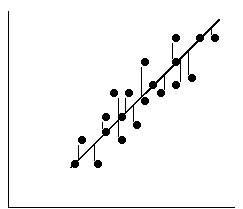
\includegraphics[height=.4\textheight]{images/regression.png}}

  \only<2>{
    \begin{displaymath}
      \min \sum (y_i-(ax_i+b))^2
    \end{displaymath}
    \vspace{1mm}
  }
  \vspace{1cm}
  \centerline{\gray{\footnotesize \url{http://www.upa.pdx.edu/IOA/newsom/pa551/Image255.gif}}}

\end{frame}

\begin{frame}
  \frametitle{Slope One : algorithm}

  Offline :
  \purple{
    \DontPrintSemicolon
    \begin{algorithm}[H]
      \For{chaque $I_i$, $I_j$}{
        $\mathcal{U} \gets \{\mbox{users who have expressed an opinion on } I_i, I_j \} $\;
        $\displaystyle
        \mbox{dev}_{i,j} \gets \frac{1}{\parallel\mathcal{U}\parallel}
        \sum_{u\in\mathcal{U}} (r_u(i) - r_u(j))$ \;
      }
    \end{algorithm}
  }
  \bigskip
  Online (for $u$) :
  \purple{
    \DontPrintSemicolon
    \begin{algorithm}[H]
      $\mathcal{V} \gets \{ j \mid u \mbox{ has expressed an opinion on } I_j \} $\;
      $\displaystyle
      r_u(i) \gets \frac{1}{\parallel\mathcal{V}\parallel}
      \sum_{u\in\mathcal{V}} (\mbox{dev}_{i,j} - r_u(j))$ \;
    \end{algorithm}
  }
\end{frame}

\begin{frame}
  \frametitle{Slope One : Regression}

  \vspace{1cm}
  \centerline{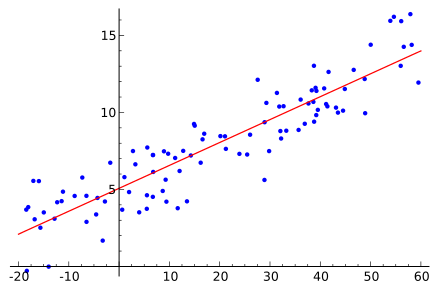
\includegraphics[height=.4\textheight]{images/linear-regression.png}}

  \vspace{1cm}
  \gray{\small "Linear regression" by Sewaqu - Own work. Licensed
    under Public domain via Wikimedia Commons -
    {\footnotesize\url{http://commons.wikimedia.org/wiki/File:Linear\_regression.svg\#mediaviewer/File:Linear_regression.svg}}}

\end{frame}

\begin{frame}
  \frametitle{Slope One : Regression}

  \vspace{1cm}
  \centerline{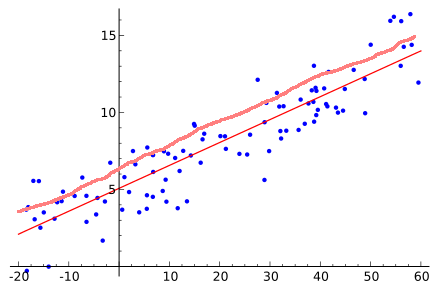
\includegraphics[height=.4\textheight]{images/linear-regression-2.png}}

\end{frame}


% ======================================================================
% Dimensionality Reduction

\begin{frame}
  \frametitle{Dimensionality reduction}

  SVD, typically $k=20\ldots 100$

  \only<1>{
    \begin{displaymath}
      M = U\Sigma V^*
    \end{displaymath}
  }
  \only<2>{
    \begin{displaymath}
      \begin{pmatrix}
        a_1 & \cdots & a_m
      \end{pmatrix}
      \begin{pmatrix}
        b_1 \\ \vdots \\ b_n
      \end{pmatrix} = \mathrm{scalar}
    \end{displaymath}
  }
  \only<3>{
    \begin{displaymath}
      \begin{pmatrix}
        a_1 \\ \vdots \\ a_m
      \end{pmatrix}
      \begin{pmatrix}
        b_1 & \cdots & b_n
      \end{pmatrix} =
      \begin{pmatrix}
        c_{1,1} & \cdots & c_{1,n} \\
        \vdots & & \vdots \\
        c_{m,1} & \cdots & c_{m,n}
      \end{pmatrix}
    \end{displaymath}
  }
  \only<4>{
    \begin{displaymath}
      \begin{pmatrix}
        a_{1,1} & a_{1,2} & a_{1,3} \\
        \vdots & \vdots & \vdots \\
        a_{m,1} & a_{m,2} & a_{m,3}
      \end{pmatrix}
      \begin{pmatrix}
        b_{1,1} & \cdots & b_{1,n} \\
        b_{2,1} & \cdots & b_{2,n} \\
        b_{3,1} & \cdots & b_{3,n}
      \end{pmatrix} =
      \begin{pmatrix}
        c_{1,1} & \cdots & c_{1,n} \\
        \vdots & & \vdots \\
        c_{m,1} & \cdots & c_{m,n}
      \end{pmatrix}
    \end{displaymath}
  }
  \only<5>{
    \begin{displaymath}
      \begin{pmatrix}
        a_{1,1} & \cdots & a_{1,k} \\
        \vdots & & \vdots \\
        a_{m,1} & \cdots & a_{m,k}
      \end{pmatrix}
      \begin{pmatrix}
        c_{1,1} & \cdots & c_{1,n} \\
        \vdots & & \vdots \\
        c_{k,1} & \cdots & c_{k,n}
      \end{pmatrix} =
      \begin{pmatrix}
        c_{1,1} & \cdots & c_{1,n} \\
        \vdots & & \vdots \\
        c_{m,1} & \cdots & c_{m,n}
      \end{pmatrix}
    \end{displaymath}
  }

\end{frame}

\begin{frame}
  \frametitle{Challenges}

  \begin{itemize}
  \item How do we measure success?
  \item What are our features?
  \end{itemize}
\end{frame}

\begin{frame}
  \frametitle{Clustering}

  \begin{itemize}
  \item kNN \only<2>{\gray{$k$-Nearest Neighbor}}
  \item Curse of Dimensionality
  \item Scalability \only<2>{\gray{$10^7$ clients, $10^6$ objets}}
  \end{itemize}
\end{frame}

%%%%%%%%%%%%%%%%%%%%%%%%%%%%%%%%%%%%%%%%%%%%%%%%%%%%%%%%%%%%%%%%%%%%%%

\talksection{Topic: Natural Language Processing}

\begin{frame}
  \frametitle{Linear Programming}
    \begin{align*}
      \text{Maximize \ } & c^T x \\
      \text{subject to \ } & Ax \le b
    \end{align*}

    \purple{Warning: this is exclusively ANN (and probably LLM) now}
\end{frame}

\begin{frame}
  \frametitle{Summarising Text}

  \only<1>{\begin{itemize}
    \item Abstractive \ \ \gray{(used to be hard, until 2018 or so)}
    \item Extractive \ \ \gray{(select sentences)}
    \end{itemize}
  }
  \only<2>{
    Challenge problem (cf. greedy solutions):
    \begin{enumerate}
    \item[] The cat is in the kitchen.
    \item[] The cat drinks the milk.
    \item[] The cat drinks the milk in the kitchen.
    \end{enumerate}
  }

\end{frame}

\begin{frame}
  \frametitle{Summarising Text}

  \only<1>{
    \begin{itemize}
    \item Sentence selection
    \item Use n-grams
    \item Stemming
    \item Stop words
    \item Prune short sentences
    \end{itemize}
  }
  \only<2>{
    \blue{Outline:}
  \begin{itemize}
  \item ILP \ \ \gray{\it(optimisation linéaire en nombres entiers)}
  \item Maximum coverage model
  \end{itemize}
  }
  \only<3>{
    \blue{ILP in canonical form:}

    \begin{align*}
      \text{Maximize \ } & c^T x \\
      \text{subject to \ } & Ax \le b \\
      & x \ge 0 \\
      & x \in \mathbb{Z}^n
    \end{align*}
  }
  \only<4-6>{
    \blue{ILP in standard form:}

    \begin{align*}
      \text{Maximize \ } & c^T x \\
      \text{subject to \ } & Ax + s = b \\
      & s \ge 0 \\
      & x \in \mathbb{Z}^n
    \end{align*}
  }
  \only<5>{\blue{This is NP hard.}}
  \only<6>{\blue{Discussion: linear vs integer programming.}}
  \only<7>{
    Let
    \begin{align*}
      c_i \text{ : } & \text{ presence of concept } i \text{ in summary} \\
      w_i \text{ : } & \text{ weight associated with } c_i \\
      l_i \text{ : } & \text{ length of sentence } i \\
      s_j \text{ : } & \text{ presence of sentence } j \text{ in summary} \\
      L \text{ : } & \text{ summary length limit } \\
      {Occ}_{ij} \text{ : } & \text{ occurence of } c_i \text{ in } s_j \\
    \end{align*}
  }
  \only<8>{
    \blue{Summarisation}

    \begin{align*}
      \text{Maximize \ } & \sum_i w_i c_i \\
      \text{subject to \ } & \sum_j l_j s_j \le L \\
      & s_j {Occ}_{ij} \le c_i, \qquad \forall i, j \\
      & \sum_j s_j {Occ}_{ij} \ge c_i \qquad \forall i \\
      & c_j \in \{0,1\}, \qquad \forall i \\
      & s_j \in \{0,1\}, \qquad \forall j
    \end{align*}
    \vspace{-1cm} % For prevwork.
  }
  \only<9>{
    Notes:
    \begin{itemize}
    \item Selecting a sentence selects all concepts it contains
    \item Selecting a concept requires it be in at least one sentence
    \item $ s_j {Occ}_{ij} \le c_i,\ \forall i, j \ \Rightarrow$
      no concept-less sentences
    \end{itemize}
  }

  \vfill
  \prevwork{Dan Gillick, Benoit Favre, \textit{A Scalable Global Model
      for Summarization}, 2009}
\end{frame}


\begin{frame}
  \frametitle{Sentiment Analysis}
  \only<1>{
    Many variations:
    \begin{itemize}
    \item Entire documents using computational linguistics
    \item Manually crafted lexicons
    \end{itemize}
  }
  \only<2>{
    Techniques
    \begin{itemize}
    \item Template instantiation\ \ \gray{(requires domain knowledge)}
    \item Passage extraction
    \end{itemize}
  }
\end{frame}

\begin{frame}
  \frametitle{Sentiment Analysis}
  \only<1-3>{
    \begin{itemize}
    \item     Extract ``opinion sentences'' based on the
      presence of a predetermined list of
      product features and adjectives.
      \only<2>{
        \begin{itemize}
        \item \blue{``The food is excellent.''}
        \item \blue{``The food is an excellent example of how not to cook.''}
        \end{itemize}
      }
    \item  Evaluate the sentences based on counts
      of positive vs negative polarity words (as
      determined by the Wordnet algorithm)
    \end{itemize}
    \only<3>{
      \blue{The good: fast, no training data, decent prediction.}

      \red{The bad: fails on multiple word sense, non-adjectives; sensitive to context.}
    }
    \vfill
    \prevwork{Hu and Lieu, Mining and Summarizing Customer Reviews, 2004}
  }
\end{frame}

\begin{frame}
  \frametitle{Sentiment Analysis}
  \only<1> {
    Words aren't enough.
    \begin{itemize}
    \item ``unpredictable plot'' vs ``unpredictable performance''
    \end{itemize}
  }

  \purple{This all changed in 2017, \textit{Attention is All You Need}, Ashish Vaswani et al., Google}

  \bigskip

  \prevwork{Turney, \textit{Thumbs Up or Thumbs Down? Semantic Orientation Applied to
      Unsupervised Classification of Reviews}, 2002}

\end{frame}


\talksection{Perceptron}

\begin{frame}{Perceptron}
  \vphrase{Gradient Descent}
\end{frame}

\begin{frame}{Perceptron}
  \begin{itemize}
  \item Supervised
  \item Binary linear classifier
  \item Online learning
  \end{itemize}
\end{frame}

\begin{frame}{Perceptron}
  \only<1>{Beginnings:
    \begin{itemize}
    \item One of first artificial neural networks (ANN's)
    \item Developed in 1957 by Frank Rosenblatt, Cornell University Aeronautical Laboratory
    \item First implemented in software (IBM 704)
    \item Intended to be a machine
    \item Designed for image recognition
    \end{itemize}}
  \only<2>{
    Controversy:
    \begin{itemize}
    \item 1958, press conference, NYT
    \item Rosenblatt too optimistic
    \item 1969, Minsky and Papert
    \end{itemize}
  }
\end{frame}

\begin{frame}{Perceptron}
  \begin{displaymath}
    f(x) = \left\{
      \begin{array}{l l}
        1 & \mbox{if } w\cdot x + b > 0 \\
        0 & \mbox{otherwise}
      \end{array}
      \right.
    \end{displaymath}

    The algorithm terminates if and only if the data is linearly
    separable.
\end{frame}

\begin{frame}{Perceptron}
  \begin{itemize}
  \item Also called ``single-layer perceptron''
  \item Not related to multi-layer perceptron
  \item Feedforward neural network
  \end{itemize}
\end{frame}

\begin{frame}{Perceptron}
  The training data is
  \begin{displaymath}
    \blue{D} = \{(x_1, y_1), \ldots, (x_n, y_n)\}
  \end{displaymath}

  \only<2->{
    \vspace{2mm}
    \blue{$x_{j,i}$} is the value of the $i$th feature of the $j$th training input vector
    
    \blue{$x_{j,0}$} = 1  \hspace{5mm} (the bias is thus $w_0$ rather than $b$)

    \blue{$w_i$} is the weight on the $i$th feature
  }
\end{frame}

\begin{frame}{Perceptron}
  Start by setting the weight vector to zero (or to some small random noise).

  \vspace{5mm}
  For each input vector $j$ in turn:
  \begin{enumerate}
  \item Compute $\hat{y} = f(w\cdot x)$
  \item Update the weights: $w_{i} = w_{i} + (y_j - \hat{y}_j) x_{j,i}$
  \end{enumerate}
\end{frame}

\begin{frame}{Multiclass Perceptron}
  \begin{displaymath}
    \hat{y} = \mbox{argmax}_y f(x, y)\cdot w
  \end{displaymath}

  \begin{displaymath}
    w = w + f(x,y) - f(x,\hat{y})
  \end{displaymath}
\end{frame}

\begin{frame}{Multiclass Perceptron: Example}
  \only<1>{\cimgh{images/pixels-to-1-class.png}}
  \only<2>{\cimgh{images/pixels-to-10-classes.png}}
\end{frame}

\begin{frame}{Perceptron History}
  \only<1>{  \begin{itemize}
    \item Perceptron is an example of SPR for image recognition
    \item Initially very promising
    \item IBM 704 \gray{(software implementation of algorithm)}\\[3mm]
    \item Mark 1 Perceptron at the Smithsonian Institution
    \item 400 photocells randomly connected to neurons.
    \item Weights encoded in potentiometers, updated during learning
      by electric motors
    \end{itemize}
    \prevwork{Frank Rosenblatt, The Perceptron: A Probabilistic Model
      for Information Storage and Organization in the Brain, Cornell
      Aeronautical Laboratory, Psychological Review, v65, No. 6,
      pp. 386–-408, 1958. doi:10.1037/h0042519}
  }
  \only<2>{
    \begin{itemize}
    \item Minksy and Papert showed perceptrons are incapable of recognizing
      certain classes of images
    \item AI community mistakenly over-generalized to all NN's
    \item So NN research stagnated for some time\\[3mm]
    \item<2> Single layer perceptrons only recognize linearly separable input
    \item<2> Hidden layers overcome this problem
    \end{itemize}
    \prevwork{M. L. Minsky and S.~A.~Papert, Perceptrons. Cambridge, MA:
      MIT Press. 1969.}
  }
  \only<3>{
    \begin{itemize}
    \item ANN's were slow.
    \item Vanishing gradient problem (Sepp Hochreiter)
    \item Support vector machines (SVN) were faster
    \end{itemize}
  }
  \only<4>{  \begin{itemize}
    \item Inputs = 400 CdS photocells
    \item Weights = potentiometers
    \item Tuning = electric motors
    \end{itemize}}
  \only<5>{\cimghh{images/mark-1-perceptron.jpg}}
  \only<6>{\cimghhhh{images/mark-1-perceptron.pdf}
    \prevwork{Frank Rosenblatt, Principles of Neurodynamics: Perceptrons
    and the Theory of Brain Mechanisms, Report No. 1196-G-8, 15 March
    1961, Cornell Aeronautical Laboratory}
  }
\end{frame}

\talksection{Neurons}

\begin{frame}{Inspired by biology}
  \cimghhh{images/tetanus-neuron.jpg}
  \centerline{\dots but only inspired}
\end{frame}

\begin{frame}
  \frametitle{Linear neuron}
  \begin{displaymath}
    y = b + \sum_i x_i w_i
  \end{displaymath}
  \only<2>{where
    \begin{align*}
      y & = \text{output} \\
      b & = \text{bias} \\
      x_i & = \text{$i^\mathrm{\,th}$ input} \\
      w_i & = \text{weight on $i^\mathrm{\,th}$ input}
    \end{align*}
  }
  \includegraphics<3>[width=.7\textwidth]{images/linear-neuron.pdf}
\end{frame}

\begin{frame}
  \frametitle{Binary threshold neuron}
  \begin{align*}
    z & = \sum_i x_i w_i \\[2mm]
    y & = \left\{
      \begin{array}{l}
        1  \text{ if } z \ge 0 \\
        0  \text{ otherwise}
      \end{array}
    \right.
  \end{align*}
  \only<2>{
    where
    \begin{align*}
      z & = \text{total input} \\
      y & = \text{output} \\
      x_i & = \text{$i^\mathrm{\,th}$ input} \\
      w_i & = \text{weight on $i^\mathrm{\,th}$ input}
    \end{align*}
    \prevwork{W. McCulloch and W. Pitts, A logical calculus
      of the ideas immanent in nervous activity. Bulletin of
      Mathematical Biophysics, 7:115--133, 1943.}
  }
  \includegraphics<3>[width=.7\textwidth]{images/binary-threshold-neuron.pdf}
\end{frame}

\begin{frame}
  \frametitle{Rectified linear neuron}
  \begin{align*}
    z & = b + \sum_i x_i w_i \\[2mm]
    y & = \left\{
      \begin{array}{l}
        z  \text{ if } z \ge 0 \\
        0  \text{ otherwise}        
      \end{array}
    \right.
  \end{align*}
  \only<2>{
    where
    \begin{align*}
      z & = \text{total input} \\
      y & = \text{output} \\
      b & = \text{bias} \\
      x_i & = \text{$i^\mathrm{\,th}$ input} \\
      w_i & = \text{weight on $i^\mathrm{\,th}$ input}
    \end{align*}
  }
  \includegraphics<3>[width=.7\textwidth]{images/rectified-linear-neuron.pdf}
\end{frame}

\begin{frame}
  \frametitle{Sigmoid neuron}
  \begin{align*}
    z & = b + \sum_i x_i w_i \\[2mm]
    y & = \frac{1}{1+e^{-z}}
  \end{align*}
  \only<2>{
    \blue{(It's differentiable!)}
  }
  \includegraphics<3>[width=.7\textwidth]{images/sigmoid-neuron.pdf}
\end{frame}

\begin{frame}
  \frametitle{Stochastic binary neuron}
  \begin{align*}
    z & = b + \sum_i x_i w_i \\[2mm]
    p &= \frac{1}{1+e^{-z}} \\[3mm]
    y & = \left\{
      \begin{array}{l}
        1  \text{ with probability } p \\[2mm]
        0  \text{ with probability } 1 - p
      \end{array}
    \right.
  \end{align*}
  \only<2>{\blue{(a probability distribution)}}

  \only<3>{\blue{Can also do something similar with rectified linear
      neurons, produce spikes with probability $p$ with a Poisson
      distribution.}}
\end{frame}

\talksection{Neural Networks}

\begin{frame}{Architecture}
  \only<1>{
    \vphrase{It's how we connect the dots (the states).}
  }
  \only<2>{Feedforward neural networks
    \begin{itemize}
    \item Flow is unidirectional
    \item No loops
    \end{itemize}

    \vspace{5mm}
    \blue{Makes linear separators (perceptron).}
  }
  \only<3-4>{\vphrase{Idea: maybe add some layers in the middle}}
  \only<4>{
    What would we put there?

    Maybe choose not to care, call them ``hidden layers''.
  }
\end{frame}

\begin{frame}{Layers}
   Neuron activity at each layer must be a non-linear function of
   previous layer

    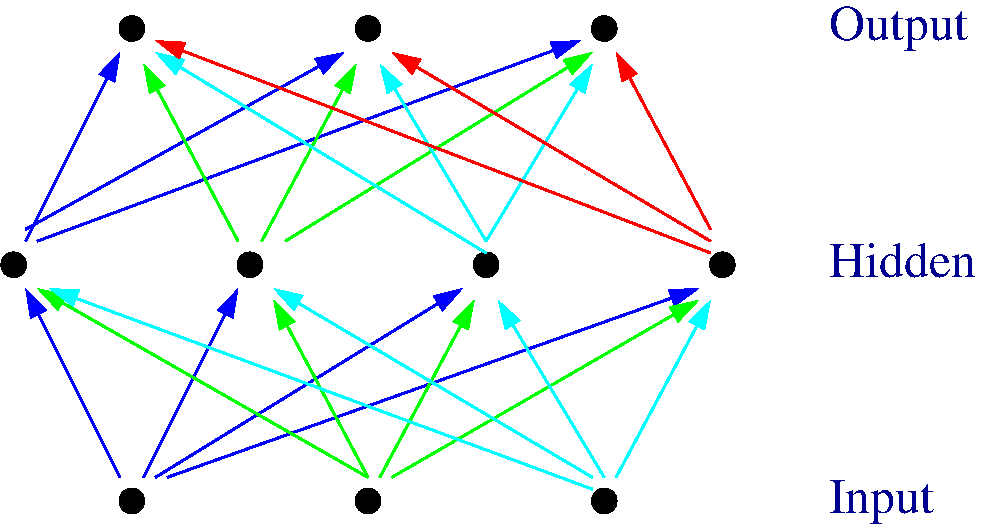
\includegraphics[width=.6\textwidth]{images/neural-network.pdf}

  \red{If more than two hidden layers, then we call it deep}
\end{frame}

\begin{frame}{Recurrent neural networks (RNN)}
  \begin{itemize}
  \item Cycles
  \item Memory
  \item Oscilalations
  \item Harder to train
  \end{itemize}
\end{frame}

\begin{frame}{Recurrent neural networks (RNN)}
\vphrase{Animated gif time}
\end{frame}

\begin{frame}
  \vphrase{So how would we train such a thing?}
  \only<2>{ It turns
    out that the perceptron algorithm is unstable and prone to many
    problems on deep or non-linear networks.}
\end{frame}

\begin{frame}
  \vphrase{Answer: Backpropagation}
\end{frame}

\begin{frame}
  \cimg{images/4layers.png}
  \centerline{$(10\times 4) + (4\times 6) + (6\times 8) + (8\times 4) = 144$ connections}
  \prevwork{Shashi Sathyanarayana, A Gentle Introduction to Backpropagation, 22 July 2014.}
\end{frame}

\begin{frame}{}
  \vspace{5mm}
  \blue{\bf Question: How do we find the weights on those 144 connections?}
    
  \only<2-3>{Need a way of refining an initial (random) guess.}
  
  \only<3>{\red{Feedforward is not stable.}}
  \only<4>{\green{So work backwards.}}
\end{frame}

\begin{frame}{Backprogation}
  \begin{itemize}
  \item Modify weights at output layer by an amount proportional to
    the partial-derivative of the error with respect to that weight.
  \item Then do next layer.
  \item Continue through all layers, recomputing partial derivatives at each step.
  \end{itemize}
  
  \only<2>{\blue{Repeat.}}
\end{frame}

\begin{frame}{Backprogation}
  \vphrase{This was hard to learn to do right.}
\end{frame}


\talksection{Backpropagation}

\begin{frame}{Backpropagation}
  \DontPrintSemicolon
  \begin{algorithm}[H]
    \SetKwFunction{algo}{algo}\SetKwFunction{proc}{proc}
    \SetKwProg{myalg}{Algorithm}{}{}
    Assign small random weights \;
    \While{not converged}{
      Feed forward to find values at each node\;
      Backpropagate to correct weights:\;
      \myalg{\algo{}}{
        Compute partial derivatives\;
        Use partial derivatives to compute gradient\;
        Use gradient to update weights (classic gradient descent)\;
      }
    }
  \end{algorithm}
\end{frame}

\begin{frame}{Backpropagation}
  Newton's Method
  \cimggg{images/newton.png}
\end{frame}

\begin{frame}{Backpropagation}
  Newton's Method
  
  \begin{displaymath}
    x_{n+1}
    = x_n - \frac{f(x_n)}{f'(x_n)}
    = x_n - \frac{f(x_n)}{\frac{\DD{f}}{\DD{x}} \big(x_n\big) }
  \end{displaymath}

  \only<2>{
    \vspace{6mm}
  or
  \begin{displaymath}
    y = \frac{\DD{f}}{\DD{x}} \Big(x_n\Big)(x-x_n) + f(x_n)
  \end{displaymath}
  }
\end{frame}

\begin{frame}
  \begin{minipage}{.5\linewidth}
    \cimgh{images/ann2.png}    
  \end{minipage}%
  \begin{minipage}{.5\linewidth}
    \begin{displaymath}
      \pdv{z}{x} = \pdv{z}{y}\pdv{y}{x}
    \end{displaymath}
  \end{minipage}
\end{frame}

\talksection{Perceptron}

\begin{frame}{Vocabulary}
  \only<1>{
    \vphrase{Activation function}

    \centerline{How the neuron decides when to fire.}
  }
  \only<2>{
    \begin{minipage}{0.5\linewidth}
      \cimg{images/sigmoid.png}
    \end{minipage}%
    \begin{minipage}{0.5\linewidth}
      \vphrase{Sigmoid}

      \vspace{1cm}
      \prevwork{\tiny By Qef (talk) - Created from scratch with gnuplot, Public Domain,\\[-3mm]
        \url{https://commons.wikimedia.org/w/index.php?curid=4310325}}
    \end{minipage}
  }
  \only<3>{
    \begin{minipage}{0.5\linewidth}
      \cimg{images/relu.png}
    \end{minipage}%
    \begin{minipage}{0.5\linewidth}
      \phrase{ReLU and Softmax}

      \vspace{5mm}
      \centerline{Rectified Linear Unit}

      \vspace{1cm}
      \prevwork{\tiny Wikimedia Commons}
    \end{minipage}
  }
  \only<4>{
    \begin{minipage}{0.7\linewidth}
      \cimg{images/max-pooling.png}
    \end{minipage}%
    \begin{minipage}{0.3\linewidth}
      \phrase{Pooling}

      \vspace{5mm}
      \centerline{max pooling}
      \centerline{downsampling}
    \end{minipage}
  }
  \only<5>{
    \begin{minipage}{0.7\linewidth}
      \cimg{images/dropout.png}
    \end{minipage}%
    \begin{minipage}{0.3\linewidth}
      \vphrase{Dropout}
    \end{minipage}
  }
\end{frame}

\talksection{Multilayer Perceptron (MLP)}

\begin{frame}{MLP}
  \begin{enumerate}
  \item Multiple layers
  \item First layer is linear
  \item Later layers use non-linear activation functions (typically sigmoid)
  \item Feedforward
  \item Can find non-linear separators
  \end{enumerate}
\end{frame}

\begin{frame}{MLP}
  \only<1>{\cimgh{images/perceptron-1.png}}
  \only<2>{\cimgh{images/perceptron-2.png}}
  \only<3>{\cimgh{images/perceptron-3.png}}
\end{frame}

\begin{frame}{MLP}
  \only<1>{\vphrase{Example: MNIST}}
  \only<2>{\vphrase{Example: simple classification tasks}}
  \only<3>{\vphrase{Example: time series}}
\end{frame}

\talksection{Recurrent Neural Networks}

\begin{frame}
  \only<1-2>{\vphrase{loops}}
  \only<2>{\centerline{so also memory}}
  \only<3>{\cimgo{images/recurrent-1.png}

    \prevwork{\url{https://colah.github.io/posts/2015-08-Understanding-LSTMs/}}
  }
  \only<4>{\cimgo{images/recurrent-2.png}

        \prevwork{\url{https://colah.github.io/posts/2015-08-Understanding-LSTMs/}}
      }
\end{frame}


\talksectionT{Convolutional Neural Networks}{ConvNets}

\begin{frame}{Tensors}
  \only<1>{
    \begin{displaymath}
      \left(
        \begin{array}{lll}
          1 & 2 & 3 \\
          4 & 5 & 6
        \end{array}
      \right)
    \end{displaymath}
  }
  \only<2>{
    \begin{displaymath}
      \left(
        \begin{array}{lll}
          \left(
          \begin{array}{l}
            1 \\ 2
          \end{array}
          \right)
       & \left(
         \begin{array}{l}
           3 \\ 4
          \end{array}
          \right) & \left(
          \begin{array}{l}
            5 \\ 6
          \end{array}
          \right) \\[5mm]

          \left(
          \begin{array}{l}
            7 \\ 8
          \end{array}
          \right) & \left(
          \begin{array}{l}
            9 \\ 10
          \end{array}
          \right) & \left(
          \begin{array}{l}
            11 \\ 12
          \end{array}
          \right)
        \end{array}
      \right)
    \end{displaymath}
  }
  \only<3>{\cimgh{images/tensor.png}}
\end{frame}

\begin{frame}{ConvNets}
  \only<1>{\vphrase{Convolutional Neural Networks}}
  \only<2>{\vphrase{The neurons are convolutions}}
  \only<3>{\cimgh{images/convnet-1.png}}
  \only<4>{\cimgh{images/convnet-2.png}}
  \only<5>{\cimg{images/convnet-3.png}}
  \only<6>{\vphrase{Example: images}}
\end{frame}


\talksection{Transfer Learning}

\begin{frame}
  \begin{itemize}
  \item Pre-trained models
  \item Only retrain the classifier at the end
  \end{itemize}
\end{frame}

\begin{frame}
  Example: PlacesVGG (2015)

  \vspace{5mm}
  
  \blue{PlacesVGG (Places2 2015)}

  \url{https://static.turi.com/models/.../places_vgg_16-1.0.tar.gz}
  
  This model is trained with VGG-16 architechture, on the Places2
  dataset. The Places2 dataset contains 8 million images of 400
  different scene categories. More details about the dataset can be
  found at http://places2.csail.mit.edu/

  \vfill
  \prevwork{\tiny\url{https://turi.com/products/create/docs/graphlab.mxnet.pretrained_image_model.html}}
\end{frame}

\talksection{Enough for Today}

\end{document}
